% arXiv working-draft format: generic APS two-column revtex4-2, deliberately no journal tag.
\documentclass[aps,twocolumn,superscriptaddress,nofootinbib,floatfix]{revtex4-2}

\usepackage{amsmath,amssymb,bm,mathtools}
\usepackage{booktabs}
\usepackage{microtype}
\usepackage{graphicx}
\usepackage{tikz}
\usetikzlibrary{arrows.meta,calc,decorations.pathreplacing,positioning}
\usepackage{xurl}
\usepackage[colorlinks=true,linkcolor=blue,citecolor=blue,urlcolor=blue]{hyperref}

\newcommand{\MSbar}{\overline{\mathrm{MS}}}
\newcommand{\mstar}{\mu_\star}
\newcommand{\alphaK}{\alpha_K}
\newcommand{\one}{\bm 1}
\newcommand{\Pd}{P_d}
\newcommand{\Pp}{P_\perp}
\newcommand{\R}{\mathbb{R}}
\newcommand{\hatm}{\widehat m}
\newcommand{\RR}{\mathcal R}

\begin{document}

\title{From the Foot Cone to Multiplicative Mass Mirrors:\\
An Involutive Reading of Charged-Fermion Mass Geometry}

\author{Andrew M. Brilliant}
\email{ab@ad-research.org}
\affiliation{Applied Dynamics Research, Sapporo, Japan}
\date{Working draft (chronicle branch) -- 28 September 2026}

\begin{abstract}
Foot's geometric reading of the charged-lepton balance places the square-root-mass vector at $45^\circ$ to the democratic direction, while Shulga's compact family cycle realizes the same balanced state from its two lowest modes. This paper reports, in the order the work was done, an attempt to read that geometry and its offshoots as involutions. The first result is exact: the equal-norm condition of the compact cycle is the null condition of the line-fixing reflection $H_3=\frac23J-I$, so the balanced state is the null set of an involution and $Q=2/3$ follows algebraically. A second exact result places the empirical mirrors on a common coordinate: for any geometric-mean mass triple the Koide statistic is $Q_3=(s-1)/(s+1)$ in the single coordinate $s=\sqrt{r}+1/\sqrt{r}$ of the geometric ratio $r$, and extended to arbitrary triples as $s_{\rm eff}=(1+Q_3)/(1-Q_3)$, the charged leptons sit at the algebraic point $s_{\rm eff}=5$ (for a non-geometric triple, a reparametrization of the Koide value $Q_3=2/3$, not an independent datum). The same involutive language was then tried on the fermion masses. The light sector inherits two geometric-mean mirrors from companion work, organized by the charged-lepton sum $\mstar$ and the constant $\alphaK=\sqrt{3/2}-1$. In the heavy sector a common renormalization scale was tried first, and nothing survived; evaluated instead at the conventional self-scale $\MSbar$ coordinates $m_c(m_c)$ and $m_b(m_b)$, with no scale adjusted; the closure is prescription-bound and disappears at every common scale we tested. The forms $m_c\simeq3\alphaK\,\mstar$ and $m_b\simeq(2+\alphaK)\,\mstar$ carry residuals of $+0.256\%$ and $-0.082\%$, and their product closes exactly on the grammar's defining constant, $m_cm_b\simeq(3/2)\mstar^2=(1+\alphaK)^2\mstar^2$. An enumeration records the contents of the declared candidate space; a late-stage procedural replay then exercises the frozen grammar on mock spectra as a check of the implemented analysis pipeline. A continuum sweep over $1$--$400$~GeV finds crossings only at undistinguished scales, and the nearest top-sector probe remains a few-percent miss within the declared grammar ($2.1\%$ above the quoted $\MSbar$ self-scale central value and $3.9\%$ below the direct determination). The heavy relation is prescribed at conventional self-scale coordinates; an explicitly transported product anchor gives it an RG-covariant continuation whose normalized residual is scale-independent by construction within a specified QCD running-and-matching prescription. This continuation does not determine why the self-scale coordinates are selected, and future mass determinations remain the empirical test of the frozen coefficients. Throughout, the reported relations are registered as pre-theoretical patterns with declared provenance, in the sense of companion work proposing explicit criteria for distinguishing structure from coincidence~\cite{BrilliantPattern}; they are offered for tracking and falsification, not claimed as physics.
\end{abstract}

\maketitle

\section{Introduction}
\label{sec:intro}

This paper is written as a chronicle. It reports a search in the order the search happened, records the misses on the same footing as the hits, and stops at the question the record poses rather than at a conclusion. The subject is the charged-fermion mass spectrum, approached through two involutive structures: a reflection in family space whose null set is the charged-lepton balance $Q=2/3$, and a reflection in logarithmic mass space whose fixed points are geometric means. Everything empirical is frozen at the PDG 2026 values~\cite{PDG2026}, so that future editions grade every relation without any adjustable element on our side.

The starting point is a recent amplitude construction. Shulga's compact family cycle~\cite{Shulga2026} builds a real amplitude from the two lowest antiperiodic modes, squares it into the periodic harmonic space $\{e^{i\phi},1,e^{-i\phi}\}$, and samples it at three equally spaced family phases, with the constant harmonic and the conjugate pair carrying equal norm. For such equal-norm states the derivation of Sec.~\ref{sec:c3} fixes the charged-lepton participation ratio at exactly $2/3$:
\begin{equation}
Q_\ell\equiv
\frac{m_e+m_\mu+m_\tau}
{\left(\sqrt{m_e}+\sqrt{m_\mu}+\sqrt{m_\tau}\right)^2}
\simeq \frac23 .
\label{eq:leprel}
\end{equation}
Foot's 1994 geometric reading identifies Eq.~\eqref{eq:leprel} with the $45^\circ$ cone of the square-root-mass vector about the democratic direction~\cite{Foot1994}. Shulga's compact-cycle construction supplies the amplitude-side realization used here, while later work developed circle-geometry and cone-selector descriptions~\cite{Kocik2012,Li2026QR}. The broader motivation is the unexplained hierarchy of the fermion Yukawa sector~\cite{PDG2026}. The ratio here uses pole masses, so no renormalization scale enters; it is in any case invariant under any common multiplicative rescaling of the three masses; the leading QED running is such a rescaling, the mass anomalous dimension being flavor-universal for three equal-charge leptons at $O(\alpha)$, and the first flavor-dependent terms enter only at two loops, at the level $O[(\alpha/\pi)^2\ln(m_\tau/m_e)]\sim{\rm few}\times10^{-5}$. With the sum $\sum_\ell m_\ell$ in the numerator, the lepton-sum scale $\mstar=\sum_\ell m_\ell$ that organizes everything below is in view from the first equation.

Two companion analyses supply the constraint space in which this paper searches~\cite{BrilliantAPPB,BrilliantMPLA}. What each manuscript of the series establishes on its own, and what the present paper imports from it, is collected in Table~\ref{tab:series} below. The first treated the lepton mass square roots as Descartes-circle curvatures and computed the fourth, outer Soddy curvature, a geometric quantity determined once the $Q=2/3$ condition is read as a Descartes condition. Under exact $Q=2/3$ its square factorizes,
\begin{equation}
\mathcal F^2=\alpha_K^2\,\mstar,
\qquad
\alpha_K\equiv\sqrt{\frac32}-1,
\qquad
\mstar\equiv m_e+m_\mu+m_\tau,
\label{eq:f2}
\end{equation}
and numerically the archived unrounded calculation gives a strange-anchor mass residual of $-0.6216\%$, reported as $-0.622\%$ throughout, under the stated PDG 2026 running prescription~\cite{BrilliantAPPB}. That paper also tested eight discrete scale prescriptions for the comparison; only $\mstar$ (and the trivially equivalent $m_\mu+m_\tau$, differing by exactly $m_e$, $0.027\%$ of the sum) produces a hit, with the conventional alternatives missing at the level recorded in Sec.~\ref{sec:enum}. The second companion showed that the compact-cycle, Descartes, and Soddy-circle descriptions are related by exact algebra as one constraint read in different coordinates, that the normalized completion is fixed on the positive exact-$2/3$ locus, and that its square $r=\alpha_K^2$ supplies the step of a geometric-mean orbit~\cite{BrilliantMPLA}. A proposed empirical cascade places the light quarks on that orbit, $\mstar\to m_s\to m_d$ with step $\alpha_K^2$, and terminates at the adopted condition $m_u^2=2m_e\,m_d$.

For the present paper it is useful to display that inherited map explicitly, because a single quadratic generates its constants. The normalized completion obeys
\begin{equation}
(1+\alphaK)^2=\frac32
\quad\Longleftrightarrow\quad
\alphaK^2+2\alphaK=\frac12,
\label{eq:quadratic}
\end{equation}
and defines
\begin{equation}
r\equiv\alphaK^2=\frac52-\sqrt6,
\qquad
M:\R_{>0}\to\R_{>0},
\qquad
M(x)=rx .
\label{eq:companionmap}
\end{equation}
Its iterates obey
\begin{equation}
x_n=M^n(x_0)=r^n x_0,
\qquad
x_n^2=x_{n-1}x_{n+1}.
\label{eq:companionorbit}
\end{equation}
Thus every interior orbit point is exactly the geometric mean of its neighbours. The map is inherited from the normalized charged-lepton completion: it is a mathematical definition, not a dynamical evolution law, and iteration introduces no additional step ratio~\cite{BrilliantMPLA}. Powers of $\alphaK$ appearing below should therefore be read as coordinates of this pre-existing multiplicative grammar rather than as exponents fitted separately to the heavy-quark masses.

One step of that cascade is the seed of the present paper. Reading the cascade as a three-slot geometric-mean relation with the strange quark as the mean and the down quark as the lower edge, solve for the upper edge: $X=m_s^2/m_d$. Evaluated at the cascade's own scale, $X=1868$~MeV against $\mstar=1883.1$~MeV, a central-value residual of $-0.8\%$, the same figure as the measured-mass upper-mirror residual of Sec.~\ref{sec:lightmirror}; evaluated at the conventional $2$~GeV reference, $X=1836$~MeV, a $-2.5\%$ miss on central values. That comparison uses central values only; as the source determinations improve, the residual itself is the summary statistic to watch. The upper slot of the light chain is therefore not a quark at all. Charm is nowhere near it ($m_c(m_c)=1273$~MeV, $m_c(\mstar)=1122$~MeV): the chain is capped from above by the charged-lepton sum, the same scale at which $\mathcal F^2$ meets the strange mass. Before any heavy-sector trial was made, the constraint space had twice returned a scale from outside the quark sector as an output. That record, not a preference, is why the search below permits independently specified physical scales, built from on-shell lepton masses, to occupy relation slots on the same footing as quark masses.

The first task of this paper is the operator form of the lepton balance. The exact-$2/3$ locus inherited from Ref.~\cite{BrilliantMPLA} posed a concrete question: is the balanced state the fixed condition of a standard operator? It is. For an $N$-channel family space define
\begin{equation}
P_N=\frac{1}{N}J,
\qquad
H_N=2P_N-I=\frac{2}{N}J-I,
\label{eq:SN}
\end{equation}
where $J$ is the all-ones matrix. Then $H_N^2=I$, and $H_N$ fixes the democratic line and negates its orthogonal complement: an orthogonal reflection across the line, related to the conventional Householder reflector by $H_N=-H_{\rm std}$~\cite{GolubVanLoan,TrefethenBau}. For $N=3$ and $x_i=\sqrt{m_i}$, the null form $x^TH_3x=0$ is exactly $Q=2/3$ (Sec.~\ref{sec:c3}), so the balanced state is the null set of the line-fixing trivalent reflection. The same operator is standard in quantum information as the Grover diffusion operator, ``inversion about the mean''~\cite{Grover1997}: the theorem the locus called for existed in the literature, and we claim no novelty for it, only for its identification with the participation-ratio null set $Q=2/N$ in the flavour context. This is why $2/3$ entered our search space at all: it is the locus the compact cycle realizes, now in operator form, not a fitted exponent.

The second task is the heavy-sector search, reported in the order in which it was performed. We first imposed a common renormalization scale, a deliberately restrictive prescription with especially clean RG properties for same-scale quark-mass ratios: nothing survives on any common-scale slice we tested (Sec.~\ref{sec:heavy}). Standard quark-mass practice then fixes the relevant methodological distinction: renormalized masses require a scheme and a reference scale, but the conventional reference prescription is not universal across quark regimes. PDG quotes the light quarks in the $\MSbar$ scheme at $2$~GeV and conventionally quotes $c$ and $b$ at $m_c(m_c)$ and $m_b(m_b)$; FLAG likewise treats several fixed charm reference scales while retaining $m_c(m_c)$ as a commonly used convention~\cite{PDG2026,FLAG2024}. Evaluated at these standard self-scale coordinates, two split closed forms hold at the per-mille level, with residuals $+0.256\%$ and $-0.082\%$, and their product closes exactly on the grammar's defining constant, $(3/2)\mstar^2$ (Sec.~\ref{sec:heavy}). We therefore adopt the following search rule throughout:
\begin{equation}
\boxed{\text{Scale dependence is allowed; scale fitting is excluded.}}
\label{eq:scalerule}
\end{equation}
Every running mass enters only under a scheme and reference-scale prescription fixed independently of the candidate relation, and no continuous renormalization scale is varied to improve closure. The declared search space was then enumerated openly and counted in full within its stated bounds (Sec.~\ref{sec:enum}), and the continuum sweep across $1$--$400$~GeV (Sec.~\ref{sec:sweep}) serves as a control on precisely the freedom that the search rule excludes. Geometric-mean and multiplicative regularities among the elementary masses have a long pedigree: the Gatto--Sartori--Tonin Cabibbo relation $\sin\theta_C\simeq\sqrt{m_d/m_s}$~\cite{GST1968,Fritzsch1978}, geometric-mean relations among quark masses~\cite{Ng1992,DSW1995}, the Georgi--Jarlskog cross-sector factors~\cite{GJ1979}, and the electroweak coincidence $m_H^2\simeq m_Z m_t$~\cite{TorrenteLujan2014}. The relations organized below differ in that every center, anchor, or coefficient is an independently specified object built from on-shell lepton masses.

Three ground rules govern everything below. First, no completeness axiom: a declared space was searched, hits and misses are reported alike, and non-participation---the top quark being the case at hand---is data, not a defect. Second, epistemic status: the empirical relations are falsifiable numerical candidates, stated now because their only decisive validation is prospective; the propagated input variations quoted later are descriptive measurement scales, not acceptance regions, $p$-values, or Gaussian significances. Third, the boundary of the newest candidates is stated precisely: the heavy forms are empirical relations prescribed at standard short-distance $\MSbar$ self-scale coordinates. Their fixed lepton-derived product anchor $(3/2)\mstar^2$ is not invariant under evolving the quark masses, but an explicitly transported anchor defines an RG-covariant continuation with an invariant normalized residual (Sec.~\ref{sec:rgtransport}); no renormalization scale is fitted to obtain the original relation. The claims below are tiered in descending strength, and the tiers do not stand or fall together: an exact reformulation (Sec.~\ref{sec:c3}); inherited light-sector identities (Sec.~\ref{sec:lightmirror}); two frozen empirical candidates (Sec.~\ref{sec:heavymirror}); documented nulls (Secs.~\ref{sec:heavy} and \ref{sec:failures}); and an open interpretation question (Sec.~\ref{sec:discussion}).


\section{The compact cycle and the trivalent reflection}
\label{sec:c3}

\subsection{$C_3$ sampling as a $1\oplus2$ decomposition}

The democratic/transverse split used throughout this section is the three-phase case of the classical symmetrical-component decomposition of polyphase systems~\cite{Fortescue1918}, built from the cube roots of unity; the zero-sequence component is the democratic line and the conjugate pair is the transverse plane. In flavour physics the same democratic decomposition underlies the tri-bimaximal mixing ansatz~\cite{HPS2002}, whose squared amplitudes $2/3,1/3,1/2$ are mixing-eigenvector components, a different invariant from the quadratic concentration $Q$ studied here, though constructed from the same machinery.

Write Shulga's real periodic amplitude in the form
\begin{equation}
Z(\phi)=s+c\,e^{i\phi}+c^*e^{-i\phi},
\label{eq:Z}
\end{equation}
with real $s$. Let $\omega=e^{2\pi i/3}$ and sample at the three family phases,
\begin{equation}
z_a=Z(2\pi a/3)=s+c\omega^a+c^*\omega^{-a},
\qquad a=0,1,2.
\label{eq:samples}
\end{equation}
The vector $z=(z_0,z_1,z_2)^T$ is real. Introduce the democratic unit vector and projectors
\begin{equation}
d=\frac1{\sqrt3}(1,1,1)^T,
\qquad
\Pd=dd^T=\frac13J,
\qquad
\Pp=I-\Pd.
\end{equation}
Because $1+\omega+\omega^2=0$,
\begin{equation}
\Pd z=s\one,
\qquad
\Pp z=(c\omega^a+c^*\omega^{-a})_{a=0}^2.
\end{equation}
Discrete orthogonality gives
\begin{equation}
\|\Pd z\|^2=3s^2,
\qquad
\|\Pp z\|^2=6|c|^2.
\label{eq:norms}
\end{equation}
Hence
\begin{equation}
\boxed{
\|\Pd z\|=\|\Pp z\|
\quad\Longleftrightarrow\quad
s^2=2|c|^2 .}
\label{eq:balance}
\end{equation}
This is the singlet/doublet balance realized in the compact-cycle construction~\cite{Shulga2026}. The phase of $c$ changes the orientation inside the transverse two-plane; it does not change the norm ratio in Eq.~\eqref{eq:norms}.

The representation structure is therefore explicit:
\begin{equation}
\R^3=E_d\oplus E_\perp\simeq\R\oplus\R^2.
\label{eq:split}
\end{equation}
The constant harmonic maps to the one-dimensional democratic sector, while the conjugate Fourier pair maps to the real transverse doublet.

\subsection{The null form is an exact reformulation of $2/3$}

For $N=3$, Eq.~\eqref{eq:SN} becomes
\begin{equation}
H_3=\frac23J-I
=\begin{pmatrix}
-\tfrac13&\tfrac23&\tfrac23\\
\tfrac23&-\tfrac13&\tfrac23\\
\tfrac23&\tfrac23&-\tfrac13
\end{pmatrix}.
\label{eq:S3matrix}
\end{equation}
It fixes the democratic direction and reverses the transverse plane. Consequently
\begin{equation}
x^TH_3x
=\|\Pd x\|^2-\|\Pp x\|^2.
\label{eq:nullform}
\end{equation}
For a general $N$-component real vector,
\begin{align}
x^TH_Nx=0
&\Longleftrightarrow 2x^TP_Nx=x^Tx\\
&\Longleftrightarrow
\frac{2}{N}(\one^Tx)^2=\sum_i x_i^2.
\end{align}
Therefore
\begin{equation}
\boxed{
x^TH_Nx=0
\quad\Longleftrightarrow\quad
\frac{\sum_i x_i^2}{(\sum_i x_i)^2}=\frac{2}{N}.}
\label{eq:generalprop}
\end{equation}
Setting $N=3$ and $x_i=\sqrt{m_i}$ gives
\begin{equation}
\boxed{x^TH_3x=0\quad\Longleftrightarrow\quad Q=\frac23.}
\label{eq:nullmirror}
\end{equation}
This is the conditional derivation used here. The representational axiom, chosen after the charged-lepton relation was known, is to read the descended $1\oplus2$ family space through its line-fixing reflection $H_3$. Shulga's compact-cycle construction supplies the equal-norm state; in the operator language that state is exactly the null condition. Once those ingredients are stated, the numerical value $2/3$ follows algebraically and is not inserted as a second parameter. The post-hoc status of the representation is therefore explicit even though the implication itself is exact.

This is a second geometric characterization of $Q=2/3$, not an explanation of why the balance holds: where the compact-cycle construction reaches the balance through Fourier amplitudes, the reflection route expresses the same balanced state as the null condition of the line-fixing involution of the $1\oplus2$ decomposition, with no harmonic coefficients to adjust. Both descriptions share the equal-norm input; neither explains why nature selects the balanced state.

Equation~\eqref{eq:nullmirror} is also Foot's geometry. If $\theta$ is the angle between $x$ and $d$,
\begin{equation}
\cos^2\theta=\frac{\|\Pd x\|^2}{\|x\|^2}.
\end{equation}
The null condition makes the democratic and transverse norms equal, so $\cos^2\theta=1/2$ and $\theta=45^\circ$: the locus of the null form is the cone introduced by Foot~\cite{Foot1994}, and we refer to it as the Foot cone throughout. Using the current charged-lepton central masses quoted by PDG, one finds $Q_\ell=0.66666446$ and $\theta=44.999905^\circ$; the small displacement from the exact cone is empirical and is not set to zero in numerical statements below~\cite{PDG2026}.

\subsection{The $N=2$ reduction}

The same family-space operator has simple lower-multiplicity limits:
\begin{equation}
H_2=\begin{pmatrix}0&1\\1&0\end{pmatrix}.
\label{eq:S21}
\end{equation}
Thus $N=2$ gives a literal exchange. The null proposition in Eq.~\eqref{eq:generalprop} should not be overextended: for $N=2$ it gives $Q_2=1$, which for positive two-component mass vectors is only reached at a degenerate boundary. The physically useful binary object is therefore the exchange operator itself, not a nontrivial two-mass cone.

We therefore treat the transition from $H_N$ to the multiplicative reflection of the next section as a change of framework rather than a natural extension: for a two-mass sector, a reflection on the logarithmic mass axis is a separate representational choice, not an object derived from the family-space cone.

\section{Multiplicative mirrors in mass space}
\label{sec:massmirror}

\subsection{Definition and unit covariance}

For any positive scale $g$, define
\begin{equation}
\RR_g(m)=\frac{g^2}{m},
\qquad
\RR_g^2=\mathrm{id}.
\label{eq:multmirror}
\end{equation}
Then $\RR_g(g)=g$, and a pair $(m_-,m_+)$ is exchanged by $\RR_g$ precisely when
\begin{equation}
m_-m_+=g^2.
\label{eq:gmrelation}
\end{equation}
In logarithmic mass coordinates, $\ell=\ln m$, Eq.~\eqref{eq:multmirror} is simply
\begin{equation}
\ell\longmapsto2\ln g-\ell,
\label{eq:logmirror}
\end{equation}
an ordinary reflection about the fixed point $g$.
Equivalently,
\begin{equation}
m_-=g\rho,
\qquad
m_+=\frac{g}{\rho}.
\label{eq:centered}
\end{equation}
Equation~\eqref{eq:gmrelation} is invariant under a change of mass units: all three masses rescale together and the equality is preserved. Its logarithmic form is ordinary reflection, Eq.~\eqref{eq:logmirror}. For any two positive masses a center $g=\sqrt{m_-m_+}$ always exists, so the involution itself carries no empirical content; the content of each candidate below is the independently specified center, anchor, or coefficient, stated in a declared convention. Throughout this paper the mirror is vocabulary; the declared object is the prediction.

\subsection{Three slots, one equation}
\label{sec:slots}

Every relation in the grammar is a three-slot object: a lower edge, a mean, and an upper edge, $m_-m_+=g^2$. Given any two, the third is determined, and the equation does not care which slot was solved for. The search below therefore assigns no positions in advance: for every triple drawn from the declared universe, each slot is solved in turn, and any member of the universe, quark mass, lepton mass, or constructed scale, may occupy any slot. In the event, the light chain fills the slots as particle, particle, scale, and the heavy candidate as particle, scale, particle; the grammar privileges neither assignment. Three consequences of that design are worth stating before the relations themselves.

First, slot freedom is what makes an anchor-in-the-center relation visible at all. Read as a mirror triple, the heavy candidate of Sec.~\ref{sec:heavymirror} has a constructed scale, $\sqrt{3/2}\,\mstar$, in the mean slot and quarks on both edges; a search restricted to all-particle triples, or with the center reserved for a particle, could never return it in this form. The mirror presentation displays a product the grammar had already fixed as its defining constant; the two one-mass forms were found as per-mass additive placements, and their product's identity with that constant was recognized afterward (Sec.~\ref{sec:heavymirror}). Second, the light chain of the companion manuscripts already used the freedom in reverse: the terminal scale was the solved slot, $P=m_u^2/m_d=2m_e$ adopted as the terminal condition before being used as an anchor~\cite{BrilliantMPLA}, so the electron-derived scale at the bottom of the light chain is a found object, not an inserted one. Third, slot freedom settles in advance where the top quark can live in this grammar: as the heaviest fermion it cannot be a mean, since no heavier edge exists, so it can only be an upper edge, requiring two points below it whose mean lands on it. Section~\ref{sec:failures} reports what that leaves for the top sector.

For presentation we sometimes use the fixed reference
\begin{equation}
P\equiv2m_e^{\rm pole},
\qquad
\widehat x\equiv x/P.
\label{eq:pairnorm}
\end{equation}
This is a coordinate convention only, but its physical inputs are declared rather than fitted: $P$ is built from the electron pole mass because the lepton anchor is a physical, pole-level object, and it is used only where a relation is tied to an absolute scale (Sec.~\ref{sec:scalegrouping}). No dynamical significance is assigned to the normalization itself. Raw running or matching calculations, where required, remain in conventional units and schemes before conversion to hatted coordinates.

\subsection{A light-sector double mirror}
\label{sec:lightmirror}

The light-sector antecedent is taken from the author's companion analyses~\cite{BrilliantMPLA,BrilliantAPPB}, where its provenance and its behavior under successive PDG editions are documented. Define
\begin{equation}
\alphaK=\sqrt{\frac32}-1.
\label{eq:alpha}
\end{equation}
The constant $\alphaK$ is not a free parameter of the quark sector: it is the normalized outer-Soddy completion of the charged-lepton Descartes configuration, fixed by the exact-$2/3$ locus alone ($\alphaK^2=5/2-\sqrt6$)~\cite{BrilliantAPPB,BrilliantMPLA}. The measured lepton masses realize that locus only approximately ($Q=2/3-2.20\times10^{-6}$, an absolute displacement), and evaluating the same completion construction at the measured masses displaces the constant by $7.3\times10^{-5}$ relative in $\alphaK^2$ ($3.6\times10^{-5}$ in $\alphaK$), negligible against every residual reported below.
The frozen light entries were
\begin{equation}
m_s^{\MSbar}(\mstar)=\alphaK^2\mstar,
\qquad
m_d^{\MSbar}(\mstar)=\alphaK^4\mstar,
\label{eq:lightclosed}
\end{equation}
where
\begin{equation}
\mstar\equiv m_e+m_\mu+m_\tau.
\end{equation}
Here $\mstar$ is an imported charged-lepton anchor in the quark sector; this paper does not derive it from quark dynamics. The anchor was not selected by scanning: $\mstar$ first appeared as the outer-Soddy completion scale of the charged-lepton Descartes configuration~\cite{Kocik2012,BrilliantAPPB}, and its role as the light-quark reference scale, including the geometric-mean cascade and its Cabibbo linkage, is developed in the companion manuscript~\cite{BrilliantMPLA}.

Equations~\eqref{eq:lightclosed} imply identically
\begin{equation}
\boxed{[m_s^{\MSbar}(\mstar)]^2=\mstar\,m_d^{\MSbar}(\mstar).}
\label{eq:uppermirror}
\end{equation}
Thus $\mstar$ and $m_d^{\MSbar}(\mstar)$ are multiplicative mirror partners about $m_s^{\MSbar}(\mstar)$:
\begin{equation}
\boxed{\RR_{m_s(\mstar)}(\mstar)=m_d(\mstar).}
\label{eq:Rupper}
\end{equation}
This is not a new fit or an independent empirical finding; it is an inherited algebraic identity, namely an exact rewriting of the inherited light closed forms~\cite{BrilliantMPLA}. The open physical question is the origin of $\alphaK$, not whether Eq.~\eqref{eq:uppermirror} follows from Eq.~\eqref{eq:lightclosed}.

A separate terminal hypothesis in the companion MPLA manuscript was
\begin{equation}
\boxed{[m_u^{\MSbar}(\mstar)]^2=P\,m_d^{\rm model}(\mstar),\qquad P=2m_e^{\rm pole},}
\label{eq:lowermirror}
\end{equation}
Here $m_d^{\rm model}$ denotes the $d$-quark mass implied by the closed-form chain of Eq.~\eqref{eq:lightclosed}, as opposed to a directly measured value. The relation is explicitly not a consequence of the cone or Descartes algebra~\cite{BrilliantMPLA}. Conditional on this additional hypothesis,
\begin{equation}
\boxed{\RR_{m_u(\mstar)}(P)=m_d^{\rm model}(\mstar).}
\label{eq:Rlower}
\end{equation}
The light sector therefore contains two linked mass-space reflections sharing the $d$ endpoint,
\begin{equation}
\boxed{
\mstar\ \xleftrightarrow[\text{center }m_s(\mstar)]{}\ m_d(\mstar)
\ \xleftrightarrow[\text{center }m_u(\mstar)]{}\ P .}
\label{eq:doublemirror}
\end{equation}
The compact notation in Eq.~\eqref{eq:doublemirror} should not obscure the different logical status of its two halves: the upper mirror follows from the inherited pair of closed forms, whereas the lower mirror uses an additional terminal hypothesis. We stress the consequence for evidential weight: because the lower mirror relates the measured $m_u$ to a \emph{model-implied} $m_d^{\rm model}$ rather than to an independently measured mass, it is an internal consistency relation of the construction, not independent empirical support for the framework, and it is not counted as such anywhere in this paper.

In pair-normalized coordinates Eq.~\eqref{eq:uppermirror} and Eq.~\eqref{eq:lowermirror} become
\begin{equation}
\widehat m_s^{\,2}(\mstar)=\widehat\mstar\,\widehat m_d(\mstar),
\qquad
\widehat m_u^{\,2}(\mstar)=\widehat m_d^{\rm model}(\mstar),
\label{eq:hattedlight}
\end{equation}
where $\widehat P=1$. The simplicity of the second expression is a coordinate convenience; the underlying raw relation remains Eq.~\eqref{eq:lowermirror}.

The dimensionless ratio implied by Eq.~\eqref{eq:lightclosed} is independent of the overall normalization and, to pure-QCD accuracy, may be compared through the same-scale light-quark ratio:
\begin{equation}
\boxed{\frac{m_s}{m_d}=\alphaK^{-2}=10+4\sqrt6=19.79795897\ldots.}
\label{eq:ratio}
\end{equation}
This ratio is the scale-invariant content of the inherited closed forms and can be stated without introducing a special running scale: QCD renormalization factors are flavor-universal and cancel exactly in quark-mass ratios, which are therefore scheme- and scale-independent up to electromagnetic corrections~\cite{GasserLeutwyler1982,PDG2026}. Its empirical standing follows the $s/d$ closed-form chain developed and tested in the companion manuscript~\cite{BrilliantMPLA}; here we record it as an inherited exact identity whose falsification route is improved lattice determinations of $m_s/m_d$; for context, FLAG 2024 quotes $m_s/m_d=20.1\pm0.3$~\cite{FLAG2024}; Eq.~\eqref{eq:ratio} differs from that central value by $-1.5\%$. We deliberately do not quote a per-mille comparison against rounded summary-table central values: the PDG summary quotes $m_s/m_d$ only as the range $17$--$22$~\cite{PDG2026}, and a significance inferred from rounded inputs with unreported correlation would be spurious. The absolute formulas in Eq.~\eqref{eq:lightclosed} are stated at $\mu=\mstar$, and this paper evaluates them there: the light-quark inputs are taken from PDG at the conventional $2$~GeV reference and run to $\mstar$ under the four-loop factor documented in Appendix~\ref{app:inputs} ($R_m=1.01750$; the same running as the companion manuscripts). With measured masses at the native scale, the inherited relations stand as follows. In the physics comparisons, a mass residual is oriented as $r_m=m_{\rm obs}/m_{\rm pred}-1$. The later census instead follows its frozen code convention $r_{\rm cell}=V/T-1$ for each grammar cell and ranks cells by $|r_{\rm cell}|$; because the assignment of value and target is class-specific, its sign is bookkeeping rather than a common physical orientation. The Monte Carlo thresholds likewise use $|r_{\rm cell}|$. The upper mirror reads $m_s^2/(\mstar m_d)-1=-0.78\%$; the scale-invariant ratio is compared only with the FLAG ratio quoted above, rather than reconstructed from rounded summary-table masses; the strange-anchor mass residual is $-0.6216\%$, reported as $-0.622\%$, against the quoted $\pm0.7$~MeV input interval; and the terminal hypothesis, evaluated with the measured $m_u(\mstar)=2.198$~MeV against the model value $2.2159$~MeV, sits at $-0.81\%$ in the mass. None of these is a fit output: the residuals below are computed from measured masses against frozen forms, and Sec.~\ref{sec:enum} counts the mirror rows as declared relations, not as enumeration discoveries.

For orientation only, the closed forms themselves give
\begin{align}
\mstar&=1883.099374\ \mathrm{MeV},\nonumber\\
m_s&=95.1158\ \mathrm{MeV},\qquad
m_d=4.80433\ \mathrm{MeV}.
\end{align}
and the terminal relation gives $m_u=2.21585$ MeV for the same inputs. These are algebraic outputs of the closed forms, not values obtained by fitting the 2026 quark masses. The lepton sum inherits its uncertainty almost entirely from the tau: from the exact pole masses $m_e=0.51099895069$ MeV, $m_\mu=105.6583755$ MeV, and $m_\tau=1776.930\pm0.090$ MeV~\cite{PDG2026}, the sum is $\mstar=1883.099374\pm0.090$ MeV, a relative uncertainty of $5\times10^{-5}$, two orders of magnitude below the per-mille residuals quoted in this paper, and negligible in every comparison we make. Every residual reported below is traceable to these exact inputs, to the quoted PDG self-scale masses, and to the frozen coefficients of Eq.~\eqref{eq:heavymirror}; no rounded intermediate is used.

\subsection{The heavy closed forms}
\label{sec:heavymirror}

The heavy-sector candidates are two one-mass closed forms, stated as relations among conventional short-distance mass coordinates with their reference coordinates stated explicitly,
\begin{equation}
\boxed{m_c\simeq 3\alphaK\,\mstar,
\qquad
m_b\simeq(2+\alphaK)\,\mstar,}
\label{eq:heavymirror}
\end{equation}
Both forms are written in the coefficient grammar of the light closed forms: every deduced mass in this paper is a small rational times an integer power of $\alphaK$ times the lepton anchor $\mstar$. The light pair used exponents $+2$ and $+4$ on that constant; the heavy pair states it in additive coordinates, charm at three $\alphaK$-units and bottom at two anchor-units plus one $\alphaK$-unit:
\begin{equation}
\frac{m_c}{\mstar}\simeq 3\alphaK,\qquad \frac{m_b}{\mstar}\simeq 2+\alphaK.
\label{eq:sharedgrammar}
\end{equation}
The defining quadratic of the whole grammar, $\alphaK^2+2\alphaK=\tfrac12$ \eqref{eq:quadratic}, gives the exact identity
\begin{equation}
2+\alphaK=\frac{1}{2\alphaK},
\label{eq:heavyidentity}
\end{equation}
and with it the product of the two forms closes on the grammar's own constant:
\begin{equation}
m_cm_b\simeq\frac32\,\mstar^2=(1+\alphaK)^2\mstar^2.
\label{eq:heavyproduct}
\end{equation}
No new number has been introduced: $3/2$ is the same constant that defines $\alphaK=\sqrt{3/2}-1$. What the construction does not determine is the factorization---the ratio
\begin{equation}
\frac{m_b}{m_c}\simeq\frac{2+\alphaK}{3\alphaK}=\frac{\alpha_K^{-2}}{6}=3.2997\ldots,
\label{eq:ratioheavy}
\end{equation}
against the measured value $3.2886$ ($-0.34\%$), is the primary empirical content of the heavy sector. The product is exact algebra once the two forms are stated; the split between them is the one number that awaits a derivation. The provenance of the pair follows the chronology of Sec.~\ref{sec:heavy}, and the two passages must be read together. The product anchor $(3/2)\mstar^2=(1+\alphaK)^2\mstar^2$ is the grammar's defining constant and was already in hand from the light-sector work; it, and the seed ratio recorded in Sec.~\ref{sec:heavy}, were the targets of the common-scale trial, which failed. The two one-mass forms were found afterward, at the self scales, as per-mass additive placements against the lepton anchor (the coefficients $3\alphaK$ and $2+\alphaK$ read off the grammar's chart one mass at a time), and only then was it noticed that their product is identically $(3/2)\mstar^2$: $3\alphaK\cdot(2+\alphaK)=3(2\alphaK+\alphaK^2)=3/2$ by Eq.~\eqref{eq:quadratic}, a recognition, not a selection step. Because the product target predates the forms, its closure is not independent evidence for them; it is the earlier candidate returning as shared algebra. Each form's empirical support is its own per-mille residual against its own mass, the heavy sector's distinguishing content remains the single factorization ratio of Eq.~\eqref{eq:ratioheavy}, and the independence claimed for the pair is prospective: the two forms are graded separately against future editions under the per-form rule stated below, so each can fail without dragging down the other. The anchor menu of Sec.~\ref{sec:enum} contains $\sqrt{3/2}\,\mstar$ because $(3/2)\mstar^2$ is the grammar's defining constant, and the census necessarily scores the product cell among its $324$ multiplicative cells; that cell records the grammar and adds no second empirical success beyond the ratio's one. The rational coefficients $3$ and $2$ are not derived from the family-space construction; they are the empirical content of the heavy candidates: the placement of the heavy masses at these fixed rational coordinates of a chart whose unit and step were fixed before the heavy-sector comparison.

The same quadratic places the heavy pair in the atlas of Sec.~\ref{sec:atlas}: the measured masses define a geometric progression $(m_c,\sqrt{m_cm_b},m_b)$ whose middle entry, $\sqrt{m_cm_b}=2308.3$~MeV against $(1+\alphaK)\mstar=2306.3$~MeV, sits at $+0.087\%$ from the lepton-derived scale. This is a reading of the candidate, not an additional hypothesis. In the companion analysis~\cite{BrilliantAPPB}, the same quadratic gives the strange prediction as $m_s^{\rm model}=\alphaK^2\mstar=(\alphaK\mstar)^2/\mstar$: the squared outer Soddy curvature, restated as one $\alphaK$-unit squared, in units of the anchor.



The comparison must keep the mass convention explicit, and here the convention is standard practice rather than an ad hoc choice. Quark masses are renormalized parameters, so a numerical mass is defined only after a scheme and reference scale are specified, and standard heavy-quark phenomenology quotes charm and bottom as the short-distance $\MSbar$ masses $m_c(m_c)$ and $m_b(m_b)$: as the PDG quark-mass review states, for the heavy quarks ``it is conventional to choose the renormalization scale equal to the quark mass''~\cite{PDG2026}. FLAG collects both $m_c(m_c)$ and $m_c(3~\mathrm{GeV})$, the former remaining a commonly used convention~\cite{FLAG2024}; precision lattice analyses report $m_{u,d,s}(2~\mathrm{GeV})$, $m_c(m_c)$, and $m_b(m_b)$ within a single calculation~\cite{Bazavov2018Masses}; and simultaneous heavy-quark determinations treat $m_c(m_c)$ and $m_b(m_b)$ together as ordinary inputs~\cite{ErlerLuo2003,KomijaniPetreczkyWeber2020}. The evaluation below uses these conventional self-scale $\MSbar$ masses, with the charged leptons at their pole masses~\cite{PDG2026}.\footnote{Heavy-quark pole masses exist perturbatively but carry infrared renormalon ambiguities of order $\Lambda_{\rm QCD}$~\cite{Bigi1994Pole,PDG2026}, so precision heavy-quark phenomenology prefers short-distance mass definitions. For charm the divergence is explicit: at $\alpha_s^{(n_f=4)}(m_c)=0.3870$, the order-by-order $\MSbar\to$pole shifts are $+209$, $+199$, and $+277$~MeV at NLO, NNLO, and N$^3$LO~\cite{MvR2000,Marquard2015}, with successive term ratios $0.95$ and $1.39$; the series diverges from its third term.} These are the same renormalization scheme at two different prescribed reference points, not a mixture of schemes. The two coordinates do sit in different effective theories, $n_f=4$ for the charm self scale and $n_f=5$ for the bottom self scale, so the candidate is a cross-threshold comparison of two conventional numbers rather than a single same-scale quantity; no threshold transport enters either coordinate itself, which is part of why the self-scale prescription is adopted (Sec.~\ref{sec:scalegrouping}). How that prescription was reached is part of the record, and Sec.~\ref{sec:heavy} reports it in order: the common-scale trial came first and failed, and the self-scale evaluation followed. Table~\ref{tab:heavy} reports the residuals and, separately, the scale obtained by propagating the uncertainties exactly as quoted by their sources. Because those sources use different confidence conventions and supply no joint covariance, the propagated variations are not combined into a confidence statement or grading boundary.

\begin{table}[b]
\caption{Split heavy-sector closed forms evaluated against the conventional PDG self-scale $\MSbar$ masses. Residuals are ${\rm observed}/{\rm predicted}-1$ with the prediction held fixed at $3\alphaK\,\mstar$ and $(2+\alphaK)\,\mstar$, respectively. Finite-difference propagation of the uncertainties as quoted by the source determinations gives fractional variations of $0.354\%$ for the charm form and $0.143\%$ for the bottom form. These values indicate the present measurement scale only: the source intervals do not share a single confidence convention and their joint covariance is unavailable, so they enter the grading rule of Sec.~\ref{sec:heavymirror} as per-form units only, not as acceptance or exclusion bands in any confidence sense. Both residuals moved slightly toward zero from the 2024 to 2026 PDG editions, but those shifts are small relative to the quoted input variations and are recorded without directional interpretation~\cite{PDG2024,PDG2026}; the edition-to-edition behavior of the antecedent relations is tracked in Ref.~\cite{BrilliantMPLA}.}
\label{tab:heavy}
\begin{ruledtabular}
\begin{tabular}{lcc}
Relation & 2024 residual & 2026 residual \\
\hline
$m_c=3\alphaK\,\mstar$ & $+0.264\%$ & $+0.256\%$ \\
$m_b=(2+\alphaK)\,\mstar$ & $-0.153\%$ & $-0.082\%$ \\
\end{tabular}
\end{ruledtabular}
\end{table}

The uncertainty and prescription questions are kept separate. Conditional on the frozen self-scale prescription $\mathcal P_{\rm self}=\{m_c(m_c),m_b(m_b)\}$, Table~\ref{tab:heavy} propagates the uncertainties quoted for the quantities entering the stated hypothesis; the two residuals share only the lepton anchor $\mstar$, whose relative uncertainty of $5\times10^{-5}$ is negligible here. The prescription itself is not a stochastic measured input, and assigning it an ``uncertainty'' would require an arbitrary probability measure over renormalization conventions. Prescription sensitivity is therefore reported separately: Sec.~\ref{sec:heavy} gives the common-scale trial, Sec.~\ref{sec:scalegrouping} evaluates alternative standard conventions, and Sec.~\ref{sec:stability} distinguishes fixed-anchor from transported-product running. Standard usage makes $m_c(m_c)$ and $m_b(m_b)$ legitimate, reproducible, same-scheme two-scale coordinates on which to state the conjecture; it does not by itself establish that their relation has dynamical significance. The claim is consequently conditional rather than convention-invariant, and the transported-product construction of Sec.~\ref{sec:rgtransport} supplies an RG-covariant continuation without selecting the initial coordinates.

The heavy forms are introduced in this paper as candidate structures in their own right, with coefficients fixed at the values displayed in Eq.~\eqref{eq:heavymirror}, and they are graded by the same rule as every other candidate in this paper: the present agreement defines the candidate, and future data grade it. The split into two one-mass forms, rather than a single product condition, is adopted so that each form can succeed or fail independently of the other. For prospective testing, the two forms of Eq.~\eqref{eq:heavymirror} stand on identical footing: their present agreement with PDG 2026 is the statement of the candidates, not their test, and the grading protocol of Sec.~\ref{sec:enum} applies to each form independently.
Frozen as numbers, with uncertainties propagated from the lepton inputs through $\mstar$ alone,
\begin{equation}
\boxed{\begin{gathered}
m_c^{\rm pred}=3\alphaK\,\mstar=1269.65\pm0.06\ \mathrm{MeV},\\
m_b^{\rm pred}=(2+\alphaK)\,\mstar=4189.4\pm0.2\ \mathrm{MeV}.
\end{gathered}}
\label{eq:frozen}
\end{equation}
These numbers will not be revised in response to future heavy-quark measurements. Each future edition will recompute the two residuals from independently updated self-scale determinations while leaving the formulas and prescription unchanged. Because each form is graded against its own quoted source scale, no joint covariance enters the grading rule. The propagated variations of Table~\ref{tab:heavy}, $0.354\%$ (charm) and $0.143\%$ (bottom) at the 2026 inputs, are recomputed from each edition's quoted uncertainties and serve as per-form grading units. The operational rule is: a form is recorded as \emph{failing} if its residual exceeds twice its current source scale in two successive editions, or if its residual grows across two successive editions while exceeding one source scale; it is recorded as \emph{converging} if its residual falls within one source scale; anything between is recorded as \emph{open}. This is a grading convention in units of each source's own quoted uncertainty, not a significance statement: the source intervals do not share a single confidence convention, so no $p$-value attaches to the rule, and the two forms are graded independently precisely so that no covariance assumption is needed. The grading units inherit the confidence conventions of their sources, so a classification can shift if reporting practice changes; recomputing the units from each edition's quoted uncertainties, rather than freezing a single interval, keeps such shifts on the record. The uncertainties displayed here are those of the predictions alone, propagated from the lepton anchor; Table~\ref{tab:heavy} separately reports the scale of the quoted heavy-quark determination uncertainties. The constant $\alphaK$ enters as the exact algebraic value of the adopted exact-$2/3$ locus, not as a measured input. The displayed prediction uncertainties, $\pm0.06$ and $\pm0.2$~MeV, propagate $\mstar$ alone. As a separate sensitivity check, replacing the exact-locus value of $\alphaK$ by the completion evaluated on the measured lepton masses would shift the predictions by approximately $46$~keV ($m_c$) and $15$~keV ($m_b$), the shift acting only on the $\alphaK$ term of each form. Those shifts are not included in the displayed uncertainties and are reported separately because they compare two definitions of the construction rather than two measurements of one input.

The relation also crosses electric-charge sectors, $Q_c=+2/3$ and $Q_b=-1/3$. No charge-selection rule is inferred from that fact. Any two positive masses possess a geometric mean; the nontrivial content here is the independently specified candidate product anchor $(3/2)\mstar^2$.

\section{The scale question: the heavy search in sequence}
\label{sec:heavy}

The heavy candidates of Eq.~\eqref{eq:heavymirror} were not found at the self scale directly, and the sequence matters: a common-scale prescription was tried first and produced nothing, and standard quark-mass practice then supplied the fixed prescription under which the candidates are stated and graded. This section reports the search in the order it happened.

\subsection{The common-scale trial}

The mirror was tried at a common renormalization scale first, a deliberately restrictive prescription: same-scale quark-mass ratios have especially clean RG properties, the common QCD renormalization factor cancelling in the ratio~\cite{GasserLeutwyler1982,PDG2026}, and the antecedent light-sector relations in the literature are stated at one scale. The first trial was the scale already in hand from the light sector, $\mstar$ itself: it produced nothing. The scan over common scales followed, and with four-loop running and threshold matching at $m_b$, inputs as in Appendix~\ref{app:inputs}, the answer is uniform. Evolved to $M_Z$, $m_cm_b=1.82$~GeV$^2$ misses $(3/2)\mstar^2$ by $66\%$, and $m_b/m_c=4.53$ misses the seed value $\alphaK^{-2}/6=3.30$ by $37\%$. At $\mu=10$~GeV the product misses by $45\%$; even at $\mu=m_b$ it misses by $27\%$. No common-scale slice we tested contains an image of the mirror. The tens-of-percent misses just displayed are the candidate relation's measured prescription sensitivity. They are reported alongside, rather than folded into, the conditional input propagation of Table~\ref{tab:heavy}: the former compares different definitions of the empirical conjecture, whereas the latter varies measured inputs within its frozen definition.

One formal crossing exists: extrapolating the four-flavor evolution of $m_b$ below threshold, $m_c(\mu)m_b(\mu)=(3/2)\mstar^2$ at $\mu\simeq2$~GeV. That point solves an equation in an unphysical continuation, since the four-flavor $m_b$ below its own threshold is not a measured bottom mass. We record the crossing and assign it no interpretation.

Two qualifications belong with this record. First, this is a documented absence, not evidence of absence: the common-scale evolution itself injects noise at the level of the effect, as $\delta\alpha_s(M_Z)=\pm0.0009$ moves $m_c(M_Z)$ by $\pm1.5\%$, four times the charm input uncertainty. Second, nothing here forbids structure at a common scale; if a common-scale derivation of the heavy relation is ever found, it will constrain the mechanism rather than compete with this reading.

\paragraph{The foliation of the heavy candidate.}
There is a geometric reason that a common-scale image of the candidate can hold at no more than one scale within each flavor-number region where the running is monotonic. Write the running of either heavy mass as $m(\mu)=m(\mu_0)\,c(\alpha_s(\mu))/c(\alpha_s(\mu_0))$. At fixed flavor number both masses share the same function $c$, so the step $\ln[m_b(\mu)/m_c(\mu)]$ is an exact invariant within each flavor-number region (Sec.~\ref{sec:stability}), and the geometric mean runs exactly like a mass,
\begin{equation}
C(\mu)\;\equiv\;\sqrt{m_c(\mu)\,m_b(\mu)}\;=\;C_0\,c\!\left(\alpha_s(\mu)\right),
\label{eq:foliation}
\end{equation}
with $C_0$ a constant. In the $(\ln m_c,\ln m_b)$ plane the common-scale flow is the translation $(x,y)\mapsto(x+t,\,y+t)$ along the direction $(1,1)$, while the constant-product loci $\ln m_c+\ln m_b=2\ln g$ are parallel lines of slope $-1$: within each flavor-number region the renormalization flow is exactly orthogonal to the leaves, and the componentwise inversion $(x,y)\mapsto(2\ln g-x,\,2\ln g-y)$---the point reflection about the leaf's center, acting on the leaf itself as the interchange of the two partners---conjugates the flow to its inverse. Both statements extend piecewise across the flavor thresholds, joined by the standard threshold matching.

\paragraph{The common-scale null.}
A common-scale realization of the candidate would therefore hold only at the single scale where a trajectory meets its leaf---a statement about one scale, not an invariant relation---and the null recorded above is the empirical fact that this meeting occurs only where at least one mass has been continued outside its physical flavor region.

\paragraph{Two scales, not one.}
Each curve carries one distinguished coordinate, the diagonal intersection $\mu=m(\mu)$ that defines the conventional self-scale mass, and the candidate below pairs the two distinct intersections $\mu_c=m_c(\mu_c)$ and $\mu_b=m_b(\mu_b)$, with $\mu_c\neq\mu_b$ in general: the candidate is a two-scale construction built from the distinguished coordinates on the two running curves, and the foliation sharpens the contrast between this self-scale construction and any common-scale trial rather than deriving one from the other. The light sector lies outside the reach of this argument: the diagonal intersections of the light quarks sit below the perturbative domain, so the construction singles out the conventional self-scale coordinates only for the heavy quarks---which is where the enumeration below begins, and which the sweep of Sec.~\ref{sec:sweep} tests against the rest of the continuum.

\subsection{From a common-scale restriction to a fixed-prescription rule}

The common-$\mu$ trial above was the first search prescription, not a theorem of admissibility. Quark masses are renormalized parameters, so a numerical mass is defined only after a renormalization scheme and reference scale have been specified, and standard practice already uses different fixed reference prescriptions in different regimes. PDG specifies light-quark $\MSbar$ masses at $\mu=2$~GeV, in part to avoid the increasing perturbative uncertainty at lower scales, whereas for charm and bottom ``it is conventional to choose the renormalization scale equal to the quark mass''~\cite{PDG2026}. FLAG makes the same point from a different computational perspective: $3$~GeV is a natural charm reference for many lattice determinations, while $m_c(m_c)$ remains sufficiently standard that both forms are collected and compared~\cite{FLAG2024}. Precision analyses likewise report light masses at $2$~GeV together with $m_c(m_c)$ and $m_b(m_b)$ in the same calculation~\cite{Bazavov2018Masses}, and simultaneous heavy-quark analyses routinely treat $m_c(m_c)$ and $m_b(m_b)$ together~\cite{ErlerLuo2003,KomijaniPetreczkyWeber2020}.

The selection criterion used here is therefore not equality of all renormalization points. It is independence of the prescription from the candidate being tested:
\begin{equation}
\boxed{\text{Scale dependence is allowed; scale fitting is excluded.}}
\end{equation}
A prescribed reference scale is part of the definition of a running-mass coordinate; a scale selected by scanning for the smallest residual would be an additional fit parameter. The former is admitted and the latter is excluded. Same-scale evaluation retains its privileged status exactly where a same-scale RG property is itself part of the claimed relation---as in the light-quark ratio of Eq.~\eqref{eq:ratio}, where the common QCD renormalization factor cancels---without becoming a universal admissibility condition on every dimensional mass relation~\cite{GasserLeutwyler1982,PDG2026}.

The light and heavy sectors satisfy this rule in different standard ways. The light-quark inputs begin at the conventional $2$~GeV reference and are evolved, where required by the inherited construction, to the independently fixed lepton scale $\mstar=1.883099$~GeV. The independently fixed $\mstar$ lies adjacent to the standard $2$~GeV light-quark reference; the proximity is context, not selection, since the lepton sum is fixed upstream by pole-mass data before any quark comparison is made. The heavy candidates use the conventional $\MSbar$ coordinates $m_c(m_c)$ and $m_b(m_b)$, the same renormalization scheme at two different prescribed reference points. The charged leptons supply pole-mass anchors, adding no QCD-running coordinate that could be adjusted against a running quark mass. No $\mu$ is determined by solving the candidate relation itself.

One asymmetry in these justifications should be stated plainly. The heavy self-scale coordinates rest on an external standard-practice basis, as documented above; the light-sector scale $\mstar$ does not: it was retained in the companion analysis after eight discrete scale prescriptions were tested and only it produced a hit~\cite{BrilliantAPPB}, so its support is provenance, not convention. Both kinds of prescription were adopted after observation, and neither is priced as selection freedom anywhere in this paper: the census of Sec.~\ref{sec:enum} counts the declared menu, not the history that produced it, and the discrete menu-growth exercise of Sec.~\ref{sec:mcnull} bounds the cost of enlarging the menu but does not reach the prescription choices themselves. What converts these post-observation adoptions into testable commitments is the prospective protocol: the prescriptions are frozen as stated, and future editions grade them without adjustment.

\subsection{The self-scale evaluation}
\label{sec:scalegrouping}

The result of the converse evaluation is Table~\ref{tab:heavy}: the candidates hold at the prescribed self-scale coordinates and at no common scale we tested. The prescription is standard rather than candidate-fitted, and it is not claimed to be uniquely compulsory: FLAG, for example, finds $3$~GeV a natural charm reference for its own presentation while retaining $m_c(m_c)$ as a commonly used convention~\cite{FLAG2024}. What the search rule requires is only that each reference point be fixed independently of the candidate relation, which the conventional self-scale prescription satisfies. The inputs group into three regimes by how they run. The charged leptons are quoted as pole masses; ``the use of OS-renormalized masses for the leptons is uncontroversial''~\cite{PDG2026}, and any short-distance prescription recovers them, so $e$, $\mu$, and $\tau$ are scale-invariant for every purpose of this paper. The light quarks are quoted at the conventional $2$~GeV reference and run perturbatively, reaching $\mu=\mstar$ with the four-loop factor $R_m=1.01750$ documented in Appendix~\ref{app:inputs}. The heavy quarks carry the theory's sharpest scale problem: ``unlike the leptons, quarks are confined, and the concept of a quark pole mass is not well-defined''~\cite{PDG2026}, so ``it is conventional to choose the renormalization scale equal to the quark mass''~\cite{PDG2026}. Charm and bottom sit in this regime. The top does not hadronize at all and behaves almost as a free quark; it is quoted as a direct reconstruction and as $m_t(m_t)$~\cite{PDG2026}. The one known geometric-mean relation involving the top, $m_H^2\simeq m_Zm_t$, is pinned to the electroweak sector, where running is mild, the scales involved differ by factors rather than orders of magnitude; whether a prescription native to that setting could extend to the QCD-dominated sectors is not obvious, and we do not assume it. One clarification closes the scale question. The closed forms are keyed relations among explicitly defined coordinates, not RG invariants: each input is taken at the reference point fixed by the search rule, so each residual is a number attached to a declared prescription rather than a value on a freely sliding scale. RG invariance is a stronger property that particular relations may possess---same-scale pure-QCD mass ratios being the case at hand~\cite{GasserLeutwyler1982,PDG2026}---not a prerequisite for a relation to be well defined. The persistence question thus has a definite answer: the fixed-center comparisons degrade when their masses alone are run, whereas the explicitly transported center of Sec.~\ref{sec:rgtransport} preserves the original normalized residual; the continuum trace of Sec.~\ref{sec:sweep} confirms that nothing closes at $M_Z$ or at any other distinguished scale along a common running path.

Two practical points fix the rest. First, the self scale is the evaluation point already conventional in heavy-quark phenomenology: quark-model determinations of $m_c$ and $m_b$ from quarkonium spectra routinely evaluate the running mass at or near the quark mass itself~\cite{PDG2026}. Second, the self-scale prescription avoids the numerically largest ambiguity in the exercise, transporting a quoted mass across a flavor threshold. At the bottom threshold the step is $\alpha_s^{(5)}(m_b)=0.22452$ against $\alpha_s^{(4)}(m_b)=0.22475$, a $0.10\%$ discontinuity; at the charm threshold the corresponding step is $0.18\%$. Evaluating each quark at its own mass crosses neither threshold.

The regime-specific prescriptions just described are load-bearing, and their weight can be quantified rather than argued. Evaluating the five declared residual equations of this paper---the strange anchor, upper mirror, and terminal relation of Sec.~\ref{sec:lightmirror} and the two heavy forms of Sec.~\ref{sec:heavymirror}---under the declared convention returns the residuals quoted above, $0.08\%$--$1.2\%$. Re-evaluating the identical frozen forms with every quark at the conventional $2$~GeV reference moves the five residuals to $2.3\%$--$17\%$; with every quark at $M_Z$, to $30\%$--$73\%$; with the FLAG charm coordinate $m_c(3\,\mathrm{GeV})=0.991(6)$~GeV substituted for $m_c(m_c)$, the charm form moves to $-21.9\%$; and with pole masses substituted for the heavy pair, the two heavy slots move to $30\%$ and $14\%$, respectively (the common-scale and pole-mass calculations use the archived running and matching prescription~\cite{BrilliantZenodoSupp}; the $3$~GeV value is from FLAG~\cite{FLAG2024}). The prescription dependence is therefore not a perturbation of the result but the difference between closure and absence, which is exactly why the convention is part of the frozen candidate definition: a common scale was tried first and its failure recorded (Sec.~\ref{sec:heavy}), the declared prescription is fixed by standard practice independently of the candidates, and prospective grading is locked to it.

\subsection{RG transport of the heavy product}
\label{sec:rgtransport}

There are two different operations that must not be conflated: moving both measured quark masses while holding the original lepton-derived product anchor $(3/2)\mstar^2$ fixed, and transporting the \emph{predicted} product together with the two quark-mass coordinates. The former generally breaks the product relation. The latter is a well-defined RG-covariant continuation of the original, self-scale empirical hypothesis. It is not an additional empirical fit or an independent explanation of why the self scales were selected.

Let $\mu_c=m_c(m_c)$ and $\mu_b=m_b(m_b)$ denote the two prescribed reference points, and let $U_c(\mu;\mu_c)$ and $U_b(\mu;\mu_b)$ be the corresponding dimensionless $\MSbar$ mass-transport factors, including any prescribed flavor-threshold matching. In a chosen common effective-theory convention, evolve the two \emph{frozen predictions} of Eq.~\eqref{eq:heavymirror} separately:
\begin{equation}
\begin{split}
 m_c^{\rm pred}(\mu)&=3\alphaK\,\mstar\,U_c(\mu;\mu_c),\\
 m_b^{\rm pred}(\mu)&=(2+\alphaK)\,\mstar\,U_b(\mu;\mu_b).
\end{split}
\label{eq:heavytransport}
\end{equation}
Consequently the predicted product must also be transported:
\begin{equation}
\boxed{m_c^{\rm pred}(\mu)\,m_b^{\rm pred}(\mu)=\frac32\,\mstar^2\,U_c(\mu;\mu_c)\,U_b(\mu;\mu_b).}
\label{eq:runningcenter}
\end{equation}
The associated multiplicative reflection is a scale-indexed family of involutions, whose squared radius is the transported product:
\begin{equation}
\mathcal R_{\mu}(m)=\frac{P(\mu)}{m},\qquad P(\mu)=\frac32\,\mstar^2\,U_c(\mu;\mu_c)U_b(\mu;\mu_b),\qquad \mathcal R_{\mu}^2=\mathrm{id}.
\label{eq:runningreflection}
\end{equation}
If the two frozen individual mass predictions held exactly at their prescribed self scales, Eq.~\eqref{eq:runningreflection} would exchange their RG-transported images at every common scale where those images are consistently defined. For the measured masses, the honest test is the normalized residual
\begin{equation}
\begin{split}
\Delta_{cb}(\mu)&\equiv\frac{m_c(\mu)m_b(\mu)}{m_c^{\rm pred}(\mu)m_b^{\rm pred}(\mu)}-1\\
&=\frac{m_c(m_c)m_b(m_b)}{(3/2)\mstar^2}-1,
\end{split}
\label{eq:rgresidual}
\end{equation}
provided the measured masses and the predicted masses use the \emph{same} linear QCD transport prescription. Thus the fractional disagreement is independent of the final common evaluation scale \emph{by construction}; numerically it is the original self-scale product residual, approximately $+0.174\%$ for the inputs adopted here. Plotting this constant at many energies would check the implementation, not provide many independent confirmations of the hypothesis. The same observation applies to the individual relative residuals.

Within a fixed active-flavor theory the two running masses share the pure-QCD mass anomalous dimension. Their common-scale ratio is then RG-invariant, and the transported product obeys the corresponding mass-running law. At heavy-flavor thresholds the effective-theory definitions and finite matching must be declared. Below bottom decoupling, a ``running bottom mass'' requires a stated formal continuation of the full-theory parameter; it is not automatically a dynamical mass in the low-energy effective theory. Electromagnetic running can also spoil exact cancellation in charm-to-bottom ratios because the two quarks carry different electric charges. We claim RG covariance of the transported construction within its specified prescription, \emph{not} scheme-independent dynamics or a new prediction from RG evolution itself.

This resolves a narrow but significant terminology issue. The original fixed-anchor comparison fails when both masses are moved without transporting the product; it is incorrect to infer that no RG-consistent transported-product formulation exists. Conversely, RG transport cannot select the original two self scales, improve the initial agreement, or rescue the hypothesis if improved self-scale masses falsify it. The common-scale null search of Sec.~\ref{sec:heavy} held the lepton-derived anchor fixed, so its negative result is compatible with the transported statement and remains part of the search record.

\subsection{Running stability}
\label{sec:stability}

The fixed-anchor diagnostic and the transported-product construction answer different questions. Holding the anchor $(3/2)\mstar^2$ fixed while evolving charm and bottom gives the failure reported in the original running test: the running product $m_c(\mu)m_b(\mu)$ drifts off the fixed anchor, since $d\ln(m_cm_b)/d\ln\mu=-2\gamma_m$ when $d\ln m_c/d\ln\mu=-\gamma_m$. That failure is retained as a check against the \emph{untransported} relation; it does not test Eq.~\eqref{eq:runningreflection}.

In contrast, the factors in Eq.~\eqref{eq:runningcenter} transport the product consistently with the two quark masses. Equation~\eqref{eq:rgresidual} shows algebraically that its normalized residual remains the original self-scale residual under matched QCD evolution. At fixed active flavor number a common-scale charm-to-bottom ratio is separately constant because the mass anomalous dimension is flavor-universal; threshold matching and the interpretation of bottom below its decoupling scale must be handled explicitly. A numerical scan therefore tests running-code consistency but does not constitute an additional set of empirical successes. The outstanding physical question is the origin, if any, of the \emph{initial} self-scale closed forms, not whether an RG transport operator can carry their proposed product.

\subsection{The continuum sweep}
\label{sec:sweep}

There remains the strongest form of the objection. A finite menu of tested scales can always be attacked as curated, while the space of possible scales is a continuum in which a determined search will manufacture agreement somewhere. We therefore swept the continuum. The enumeration universe is the six quarks, the three charged leptons, and nine discrete anchors; the running masses are tabulated on a logarithmic grid over $1$--$400$~GeV, every ordered pair of distinct masses ($18\times17$) is paired with a distinct third object for the remaining slot ($16$ choices), in either mirror orientation ($\times2$), minus four excluded self-matching configurations, giving $2\times18\times17\times16-4=9788$ geometric-mean configurations, each scanned for zero crossings of its residual along the grid.

The sweep records 360 crossings. Ninety-two of them involve a mass continued outside its physical regime, the charm--bottom product crossing at $\mu=2.069$~GeV among them, matching the unphysical continuation recorded in the common-scale trial. The remaining 268 sit at undistinguished $\mu$ between running curves, and are guaranteed by continuity whenever a prediction falls inside a mass's running range: they are the generic coincidences the objection predicts, and they occur at meaningful places no more often than anywhere else. No crossing lands at a distinguished scale. The tolerance in the scale coordinate is defined as the census window applied to scales: a crossing at $\mu_{\rm cross}$ is counted as landing at a distinguished scale $\mu_0$ only if $|\mu_{\rm cross}-\mu_0|/\mu_0<5\times10^{-3}$. Under that criterion, no crossing sits at $M_Z$, $m_c$, $m_b$, $m_t$, or $\mstar$. The null has a quantitative baseline: were the $360$ crossings distributed uniformly in $\ln\mu$ over the swept range, the five windows, each of relative half-width $5\times10^{-3}$, would collect about $3$ of them by chance; none is observed. The configurations internal to the anchor menu produce no crossings at all; their nearest misses are the expected near-identities, $(3/2)\mstar^2=\frac32\mstar^2$ exact by construction and the arithmetic-geometric pair at $-0.084\%$, arithmetic among derived quantities, ranking separately from every mass-involving comparison. The distinction the sweep draws is between a zero of an equation, which continuity guarantees somewhere, and a zero at a distinguished point, which it does not: the declared relations all live at the second kind of point, and the sweep finds that such points are where the crossings are not. The sweep is thus the control on precisely the freedom that the search rule excludes: it is not scale dependence that disqualifies a candidate, but the use of a scanned scale as a discovery instrument. Evaluated instead at the declared regime-native coordinates of Sec.~\ref{sec:scalegrouping} (self scales for the heavy quarks, $\mstar$ for the light quarks), the same universe returns the six sub-$1\%$ cells itemized in Sec.~\ref{sec:enum}: the heavy candidate, two Descartes relations (one represented twice because $m_\tau$ is both a mass and an anchor), and the two measured-mass images of declared light relations. The complete crossing and nearest-miss tables, the input grid, and its checksum are archived with the enumeration code and the supplementary calculations~\cite{BrilliantGitHubEnum,BrilliantZenodoSupp}.

\section{What the mirror grammar does not explain}
\label{sec:failures}

\subsection{The up-type triple is not another balanced $C_3$}

The charged-lepton value $Q_\ell\simeq2/3$ was first reported by Koide~\cite{Koide1983}; the Foot-cone and compact-cycle formulations used above are geometric and amplitude readings of that empirical relation. We introduce the conventional name only here because the argument to this point depends on the balance, the cone, and the reflection operator rather than on its historical label.

A tempting extension is to impose the same trivalent balance on $(u,c,t)$. It fails. For any three positive square-root coordinates $v_j=\sqrt{m_j}$ (not the masses $m_j$ themselves) written in the standard circulant form~\cite{Koide1983,Zenczykowski2012}
\begin{equation}
v_j=A\left[1+\sqrt2\,k\cos\left(\frac{2\pi j}{3}+\delta\right)\right],
\end{equation}
the participation ratio is
\begin{equation}
Q_v\equiv\frac{\sum_jv_j^2}{(\sum_jv_j)^2}=\frac{1+k^2}{3}.
\label{eq:Qk}
\end{equation}
The proof is immediate from $\sum_j\cos\theta_j=0$ and $\sum_j\cos^2\theta_j=3/2$ for $\theta_j=2\pi j/3+\delta$:
\begin{align}
\sum_j v_j^2&=3A^2(1+k^2),
&
\sum_j v_j&=3A,
\nonumber\\
Q_v&=\frac{3A^2(1+k^2)}{9A^2}
=\frac{1+k^2}{3}.
\end{align}
Thus the self-dual point is $k=1$, where $Q_v=2/3$ is the Koide value, independent of the phase $\delta$. The phase fixes the azimuth in the transverse plane; it cannot repair the polar norm imbalance. This participation-ratio consequence is implicit in the circulant analysis of \.{Z}enczykowski~\cite{Zenczykowski2012} and is recorded here only to fix notation.

Using the common full-SM $\MSbar$ Yukawas at $M_Z$ reported by Antusch, Hinze, and Saad~\cite{Antusch2026},
\begin{equation}
(y_u,y_c,y_t)=(7.04\times10^{-6},\,3.56\times10^{-3},\,0.967),
\end{equation}
we obtain directly
\begin{equation}
k_{uct}^{\rm dir}=1.2895,
\qquad
k_{uct}^{\rm inv}=1.3196,
\label{eq:upfail}
\end{equation}
where the direct coordinate uses $v_i=\sqrt{y_i}$ and the reciprocal coordinate uses $v_i=1/\sqrt{y_i}$. Equation~\eqref{eq:Qk} then gives $Q_{uct}^{\rm dir}\simeq0.888$ and $Q_{uct}^{\rm inv}\simeq0.914$, both far from $2/3$. Neither coordinate is close to the self-dual value. $Q_v$ is invariant under any common rescaling of the three Yukawas, and no scheme choice is used here to move $k$ toward $1$; the five-order-of-magnitude span of $(y_u,y_c,y_t)$, compared with the charged-lepton span of only $\sim3500$, makes a balanced up-type $C_3$ description implausible on basic dimensional grounds before any computation. Differential running does not rescue it either. At one loop the gauge and trace contributions to the up-type Yukawa anomalous dimensions are flavor-universal and cancel in ratios, leaving
\begin{equation}
16\pi^2\,\frac{d}{d\ln\mu}\ln\frac{y_t}{y_c}
=\frac32\Big[y_t^2-y_c^2-\sum_j\big(|V_{tj}|^2-|V_{cj}|^2\big)\,y_{d_j}^2\Big]
\simeq\frac32\,\big(y_t^2-y_b^2\big),
\label{eq:drift}
\end{equation}
which evaluates to $+1.40$ at $M_Z$ (the CKM down-sector terms contribute only $-4\times10^{-4}$): the residual scale dependence of $Q_{uct}$ is the top Yukawa talking to itself, and its sign carries $Q_{uct}$ \emph{away} from $2/3$ as the scale increases. We record for completeness that the direct value sits near a different rational, $9Q_{uct}^{\rm dir}=7.9886$, within $0.15\%$ of $8$. That proximity is a running-scale crossing, not a fixed point: interpolation of the tabulated couplings of Ref.~\cite{Antusch2026} places $9Q_{uct}=8$ at $\mu\simeq2.2$~TeV (one-loop integration: $2.7$~TeV), above which the ratio departs upward, and the crossing scale is exponentially sensitive to inputs (a $\pm0.35\%$ shift in $y_t$ moves it by factors between $0.6$ and $1.8$), so no sharp scale target can be quoted for it. The same flat-curve instability afflicts the high-scale crossing of Ref.~\cite{Rivero2026} discussed below. We claim nothing for the value $8/9$ itself. We therefore do not introduce a new angle, scale, or branch to rescue an up-type $C_3$ mirror. We note for completeness that a direct attempt to extend the compact-cycle Fourier construction itself to the quark triples does not succeed: when the balance is not clean, the harmonic coefficients become adjustable parameters that cannot be derived, which is precisely the freedom the reflection language of Sec.~\ref{sec:c3} does not possess. This failure is part of the motivation for the $3+2+1$ slicing of Sec.~\ref{sec:atlas}.

The same failure is visible in the prior literature, where quark-sector Koide ratios reach $2/3$ only under conventions the present paper excludes. The strange--charm--bottom tuple requires a signed (negative) square root for the strange quark~\cite{Rivero2011}. The heavy triple $(c,b,t)$ approaches $0.669$ in treatments that evaluate the heavy quarks at pole-style masses while the lighter members enter as running masses~\cite{Cao2012,RodejohannZhang2011}, a convention mix the present paper excludes; the observation was noted in the preprint of Ref.~\cite{RodejohannZhang2011} and withdrawn from its published version. The inverse-shape down-sector rule of Ref.~\cite{Rivero2026} does reach $2/3$ under full Standard Model running, and its residual is sub-tolerance over a broad scale range precisely because the ratio is nearly scale-insensitive; the price is that the crossing scale, quoted near $280$~TeV, inherits the full uncertainty of the input masses, so no sharp prospective target can presently be defined for other triples converging there. For the up-type charge triple considered here, by contrast, no declared convention yields $2/3$: reported values sit near $0.89$, and in our regime-native conventions Eq.~\eqref{eq:upfail} gives $0.888$ direct and $0.914$ reciprocal.

This negative result is useful. In the present organization, $u$, $c$, and $t$ need not form one self-dual triplet. They occupy different roles in the $3+2+1$ bookkeeping discussed below: $u$ is the center of a conditional light-sector mirror, $c$ is one edge of the heavy candidate pair, and $t$ is a singleton.

\subsection{The top sector is a structural null}
\label{sec:topnull}

The slot grammar of Sec.~\ref{sec:slots} explains why the top quark has no mirror partner in this framework. As the heaviest fermion it can occupy only the upper edge of a three-slot object: nothing heavier exists to bound it from above, so its center would have to be built from two points below. The quark pairs offer no working combination. The continuum sweep of Sec.~\ref{sec:sweep} quantifies this: under every scale convention tested, no pair drawn from $(u,d,s,c,b)$ produces a center near the top scale. The integer-exponent grammar fails separately, and we record its nearest approach.
\begin{equation}
m_t\stackrel{?}{=}\alphaK^{-3}\mstar=8\,(2+\alphaK)^3\mstar=165.88\ \mathrm{GeV},
\label{eq:topprobe}
\end{equation}
and it fails. The value sits between the two conventional PDG top masses: $3.9\%$ below the direct determination $m_t=172.60\pm0.27$ GeV and $2.1\%$ above the $\MSbar$ value $m_t(m_t)=162.5^{+2.1}_{-1.5}$ GeV extracted from the $t\bar t$ cross section~\cite{PDG2026}, while those two scheme values themselves differ by $6.2\%$. The probe lies outside each quoted central interval, but only $3.38$~GeV above the $\MSbar$ central value compared with its quoted $+2.1$~GeV upper uncertainty; it is therefore a few-percent miss, not a decisive exclusion. No small rational coefficient repairs it without post-hoc fitting. Nor can the comparison be repaired by running. Below its own mass the top decouples from the effective theory in which the lighter quarks are measured, and the evolution from there downward is flavor-universal: carried to a common low scale in two internally consistent pipelines, the up-type ratio returns $7.9889$ and $7.9900$, frozen at its decoupling value and identical at $m_b$, $2$~GeV, and $\mstar$; an evolved $m_t(\mu)$ at a common lower scale is a constant extrapolation, carrying no information beyond the high-scale inputs. Landing exactly on $9Q_{uct}=8$ at any such scale would require $m_t(m_t)\simeq166.4$~GeV, $2.4\%$ above the measured $\MSbar$ value and outside its quoted uncertainty---a bookkeeping target, not a datum. We document Eq.~\eqref{eq:topprobe} as a negative result and decline to speculate on how the pole and $\MSbar$ top determinations will converge as the measurements improve. No coefficient on our side is adjustable in response: future determinations either move toward $165.88$ GeV or they do not.


The only two points below the top that do produce a geometric-mean center at its scale are electroweak. The combination $m_t=m_H^2/m_Z$ evaluates to $171.9$~GeV, within half a percent of the direct determination $m_t=172.60\pm0.27$~GeV, and Torrente-Luj\'an has already noted a relation of this form~\cite{TorrenteLujan2014}. We report it as a pointer, not a claim: the Higgs and $Z$ masses belong to a different sector, and no common geometry linking them to the lepton-sum scale is exhibited here. Within the fermion mass space this paper enumerates, the top is a singleton. Whether that is a defect of the grammar or a datum about it is left open.
\subsection{No topological inversion}

The two-sheeted $4\pi\to2\pi$ language of the compact cycle does not by itself yield a reciprocal mass coordinate. The antiperiodic deck transformation is a sign change upstairs; the symmetric square removes that sign, so within the present construction we obtain no route to $m\mapsto1/m$. Such a coordinate remains available as a separate involutive representation; we simply do not derive it here.

\section{A $3+2+1$ mirror atlas}
\label{sec:atlas}

The surviving structures can be displayed without claiming that they share one dynamics. The quark slicing $(u,d,s)+(c,b)+t$ used here is phenomenological bookkeeping inherited from the antecedent mass relations; it is not a Standard-Model representation decomposition. This light/heavy/top slicing is also the standard organizing structure of quark mass-matrix texture analyses~\cite{FritzschXing2000}. The tiers are connected only through physical lepton scales: no relation in this paper equates a light-quark mass to a heavy-quark mass or compares them at a common renormalization scale, and every cross-regime anchor ($\mstar$ in the light sector, $\sqrt{3/2}\,\mstar$ in the heavy sector) is built from on-shell lepton masses, the one sector where pole masses are uncontroversial~\cite{PDG2026}. The lepton anchor removes a second adjustable QCD-running coordinate from each comparison; it does not render the quark-side coordinates scheme-independent, and no such invariance is claimed. Figure~\ref{fig:atlas} separates the exact family-space statement from the mass-space relations.

\begin{figure*}[t]
\centering
\begin{minipage}[t]{0.48\textwidth}
\centering
\textbf{(a) Charged leptons: trivalent family reflection}\\[2pt]
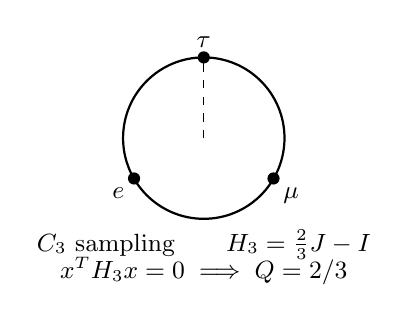
\begin{tikzpicture}[>=Latex,x=0.82cm,y=0.82cm,font=\small]
\draw[thick] (3,2.0) circle (1.25);
\coordinate (A) at (3,3.25);
\coordinate (B) at (1.92,1.375);
\coordinate (C) at (4.08,1.375);
\fill (A) circle (2.2pt) node[above] {$\tau$};
\fill (B) circle (2.2pt) node[below left] {$e$};
\fill (C) circle (2.2pt) node[below right] {$\mu$};
\draw[dashed] (3,2.0)--(A);
\node[align=center] at (3,0.15) {$C_3$ sampling\qquad $H_3=\frac23J-I$\\[-1pt]
$x^TH_3x=0\;\Longrightarrow\;Q=2/3$};
\end{tikzpicture}
\end{minipage}\hfill
\begin{minipage}[t]{0.48\textwidth}
\centering
\textbf{(b) Light sector: two linked mass reflections}\\[2pt]
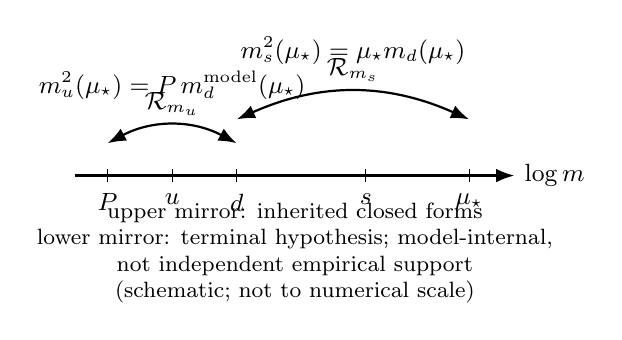
\begin{tikzpicture}[>=Latex,x=0.82cm,y=0.82cm,font=\small]
\draw[->,thick] (0.25,1.55)--(7.05,1.55) node[right] {$\log m$};
\foreach \x/\lab in {0.75/$P$,1.75/$u$,2.75/$d$,4.75/$s$,6.35/$\mu_\star$}{
  \draw (\x,1.45)--(\x,1.65);
  \node[below] at (\x,1.42) {\lab};
}
\draw[<->,thick] (0.75,2.05) to[bend left=28] node[above] {$\mathcal R_{m_u}$} (2.75,2.05);
\node[above] at (1.75,2.58) {$m_u^2(\mu_\star)=P\,m_d^{\rm model}(\mu_\star)$};
\draw[<->,thick] (2.75,2.42) to[bend left=24] node[above] {$\mathcal R_{m_s}$} (6.35,2.42);
\node[above] at (4.55,3.12) {$m_s^2(\mu_\star)=\mu_\star m_d(\mu_\star)$};
\node[align=center,font=\footnotesize] at (3.65,0.35) {upper mirror: inherited closed forms\\lower mirror: terminal hypothesis; model-internal,\\not independent empirical support\\(schematic; not to numerical scale)};
\end{tikzpicture}
\end{minipage}

\vspace{0.6em}

\begin{minipage}[t]{0.48\textwidth}
\centering
\textbf{(c) Heavy sector: binary mass mirror}\\[2pt]
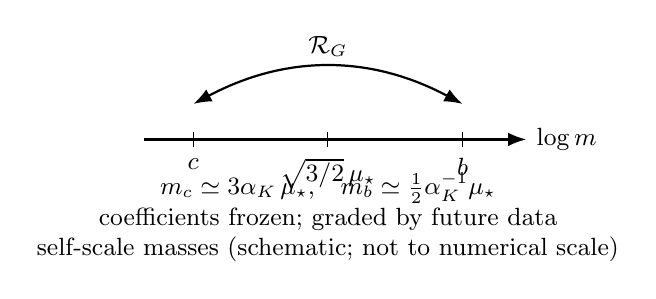
\begin{tikzpicture}[>=Latex,x=0.9cm,y=0.9cm,font=\small]
\draw[->,thick] (0.45,1.55)--(5.85,1.55) node[right] {$\log m$};
\foreach \x/\lab in {1.15/$c$,3.05/$\sqrt{3/2}\,\mstar$,4.95/$b$}{
  \draw (\x,1.45)--(\x,1.65);
  \node[below] at (\x,1.42) {\lab};
}
\draw[<->,thick] (1.15,2.05) to[bend left=28] node[above] {$\mathcal R_G$} (4.95,2.05);
\node[align=center] at (3.05,0.45) {$m_c\simeq3\alphaK\,\mstar$,\quad $m_b\simeq\frac12\alphaK^{-1}\mstar$\\coefficients frozen; graded by future data\\self-scale masses (schematic; not to numerical scale)};
\end{tikzpicture}
\end{minipage}\hfill
\begin{minipage}[t]{0.48\textwidth}
\centering
\textbf{(d) Top sector: singleton}\\[2pt]
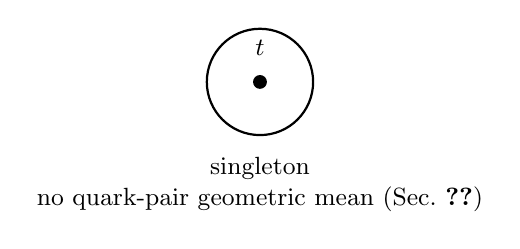
\begin{tikzpicture}[x=0.9cm,y=0.9cm,font=\small]
\draw[thick] (3.0,2.0) circle (0.75);
\fill (3.0,2.0) circle (2.5pt) node[above=6pt] {$t$};
\node[align=center] at (3.0,0.55) {singleton\\no quark-pair geometric mean (Sec.~\ref{sec:topnull})};
\end{tikzpicture}
\end{minipage}
\caption{An involutive ``atlas'' rather than a unified dynamical model. The charged-lepton panel is the exact family-space result derived from the compact-cycle $1\oplus2$ decomposition. The light and heavy panels are schematic mass-space relations on logarithmic axes; horizontal positions are not plotted to numerical scale. Within the light panel the two arrows differ in status: the upper mirror is an inherited algebraic identity whose measured-mass image is compared separately with data, while the lower mirror's endpoint is the model-implied $m_d^{\rm model}$ (Sec.~\ref{sec:lightmirror}). Their visual similarity does not identify the underlying operators; it displays the question being asked.}
\label{fig:atlas}
\end{figure*}

The pattern can be summarized in words rather than as an equation: the specific quark architecture considered here contains two linked internal multiplicative mirrors in the light sector, one candidate product closure in the heavy pair, and no nontrivial internal flavor reflection for the singleton. This $3+2+1\to2+1+0$ count is an organizational observation, not a group-theoretic theorem. In particular, the two light mirrors are not forced merely because three light masses exist; they arise from the specific antecedent equations \eqref{eq:lightclosed} and \eqref{eq:lowermirror}.

The lepton side is structurally different. Its ``mirror'' is the family-space reflection operator $H_3$, and the empirical mass vector lies approximately on its null cone. The light and heavy quark mirrors instead act on positive mass coordinates by inversion about geometric-mean fixed points. The central open question is therefore not whether the matrices are literally the same. They are not. It is whether the repeated appearance of involutive decompositions is a useful guide to a future representation-theoretic calculation.

\subsection{One coordinate for every mirror triple}
\label{sec:gpkoide}

The atlas of the preceding section displays four mass-space triples and asks whether their repeated involutive form is more than bookkeeping. For geometric-mean triples the answer is exact, and it collapses the Koide content of every such triple into a single number. Any mirror triple is by definition a geometric progression: $m_-\,m_+ = m_0^2$, with ratio $r = m_+/m_0 \geq 1$. Define the symmetric coordinate
\begin{equation}
s \;=\; \sqrt{r} + \frac{1}{\sqrt{r}} \;\geq\; 2 ,
\label{eq:sdef}
\end{equation}
with equality if and only if the triple is democratic ($r=1$). Writing the triple as $(m_0/r,\,m_0,\,m_0 r)$, the common scale $m_0$ cancels in the Koide statistic $Q_3 = (\sum_i m_i)/(\sum_i\sqrt{m_i})^2$, giving $Q_3 = (r^{-1}+1+r)/(r^{-1/2}+1+r^{1/2})^2$; since the denominator is $(s+1)^2$ and the numerator is $s^2-1$, one obtains
\begin{equation}
Q_3 \;=\; \frac{s-1}{s+1},
\qquad\text{equivalently}\qquad
s \;=\; \frac{1+Q_3}{1-Q_3} .
\label{eq:q3s}
\end{equation}
The same substitution gives the pair statistics and the floor deviations,
\begin{equation}
Q_2^{\mathrm{mean}} = \frac{s}{s+2},
\qquad
Q_2^{\mathrm{outer}} = 1 - \frac{2}{s^2},
\qquad
2Q_2 - 1 = \frac{s-2}{s+2},
\qquad
3Q_3 - 1 = \frac{2(s-2)}{s+1} ,
\label{eq:q2forms}
\end{equation}
the two mean pairs being equal by the reflection symmetry $r\leftrightarrow 1/r$. Equation~\eqref{eq:q3s} maps integer $s$ to unit fractions: $s=2\leftrightarrow Q_3=1/3$ (the democratic floor), $s=3\leftrightarrow 1/2$, $s=5\leftrightarrow 2/3$ (the Koide value), $s=7\leftrightarrow 3/4$. The coordinate $s$ therefore linearizes the entire Koide content of any geometric-mean triple into one number, and the inverse map in Eq.~\eqref{eq:q3s} places even non-geometric triples on the same ladder through the effective coordinate $s_{\mathrm{eff}}=(1+Q_3)/(1-Q_3)$.

\begin{table}[t]
\centering
\caption{Mirror triples in the coordinate $s$ of Eq.~\eqref{eq:sdef}. Non-geometric triples (leptons, EW) use $s_{\mathrm{eff}}=(1+Q_3)/(1-Q_3)$, a reparametrization of $Q_3$. Light-cascade row: model $s$ and model $Q_3$; measured $Q_3=0.64897$ gives $s_{\mathrm{eff}}\simeq4.698$.}
\label{tab:sladder}
\begin{tabular}{lcc}
\toprule
Triple & $s$ & $Q_3$ \\
\midrule
Charged leptons $(e,\mu,\tau)$ & $4.99996$ & $0.66666446$ \\
Light cascade $(m_d, m_s, \mstar)$ & $4.67424$ & $0.64753$ \\
Heavy doublet $(m_c,\sqrt{m_cm_b},m_b)$ & $2.0897$ & $0.3527$ \\
EW triple $(W, Z, t)$ & $2.0466$ & $0.3434$ \\
Terminal cascade $(P, m_u, m_d)$ & $2.1516$ & $0.3654$ \\
\bottomrule
\end{tabular}
\end{table}

Table~\ref{tab:sladder} places the triples of this paper and its companions on the one coordinate. The leptons sit at the exact algebraic point $s=5$ at $-0.0009\%$; the heavy doublet, the electroweak triple, and the terminal cascade cluster at the democratic floor $s\simeq2.05$--$2.15$; and the light cascade sits at the intermediate point $s=4.67424$, the mirror-side value closest to the leptons'. For the light cascade the model triple $(m_d, m_s, \mstar)$ with $m_s^2=\mstar m_d$ is a geometric progression with step $r=\alphaK^{-2}$, so taking the model inputs as exact, Eq.~\eqref{eq:sdef} gives the closed form
\begin{equation}
s_{\mathrm{light}} = \alphaK^{-1} + \alphaK = \frac{2+3\sqrt{6}}{2},
\label{eq:slightclosed}
\end{equation}
and substitution into Eqs.~\eqref{eq:q3s}--\eqref{eq:q2forms} gives closed radical forms, e.g.\ $Q_3 = 3(9-2\sqrt{6})/19$ and $Q_2^{\mathrm{mean}}=(7-2\sqrt{6})/3$. These forms are exact statements about the \emph{model} triple. With physical masses ($m_d(\mstar)=4.78$~MeV, from the $2$~GeV value $4.70$~MeV under $R_m=1.01750$), the measured $Q_3=0.64897$ deviates from the closed form $0.64753$ by $0.22\%$; the closed forms are quoted as properties of the model, not as exact fits to data.

One further reading is available, and the axioms of this series were written to keep it open: the candidate space was declared over anchors and geometric means without presuming the Standard Model spectrum to be complete. Equation~\eqref{eq:q3s} is a statement about geometric progressions, indifferent to whether the middle entry of a mirror triple is a measured mass or a derived center. Under this inverse reading, the heavy-triple row of Table~\ref{tab:sladder} records: should a state be found at the center $\sqrt{3/2}\,\mstar=2.306$~GeV, it would join the progression $$(m_c,\sqrt{m_cm_b},m_b)$$ at $s=2.0897$ and inherit the closed forms of Eqs.~\eqref{eq:q3s}--\eqref{eq:q2forms} without disturbing any declared relation. We record this as an exact property of the grammar, not as a prediction: the $2.3$~GeV region is densely measured (open-charm thresholds, $D$-meson spectroscopy), the measured spectrum there offers no candidate, and the point was checked and set aside; any occupant would have to be established on experimental grounds independent of the mirror grammar. The geometry supplies the coordinate; it does not manufacture the occupant.

\section{Logical status and falsification}

The main risk in empirical mass geometry is to blur identities, fits, and interpretations. Table~\ref{tab:status} states the standing of each ingredient used here.

\begin{table*}[t]
\caption{Logical status of the main statements. ``Conditional identity'' means exact algebra once the stated antecedent hypothesis is accepted. Entries marked $\dagger$ involve cross-sector or prescription-specific comparisons: lepton-derived anchors imported into the quark sector, or factors evaluated at different prescribed renormalization points. Complete covariance information across such boundaries awaits future publication; the stated accuracies of these entries are descriptive and provisional, registered pending that data rather than quoted as significance statements (see the epistemic-status paragraph of the Introduction).}
\label{tab:status}
\begin{ruledtabular}
\begin{tabular}{p{0.30\textwidth}p{0.24\textwidth}p{0.35\textwidth}}
statement & basis & standing \\
\hline
$H_N=2P_N-I$, $H_N^2=I$ & linear algebra & proposition \\
$x^TH_Nx=0\iff \sum x_i^2/(\sum x_i)^2=2/N$ & Eq.~\eqref{eq:generalprop} & proposition \\
Shulga equal norm $\Rightarrow Q_\ell=2/3$ after $C_3$ sampling & compact-cycle antecedent + proposition & conditional derivation \\
$m_s^2(\mstar)=\mstar m_d(\mstar)$$^\dagger$ & inherited $m_s(\mstar)=\alpha_K^2\mstar$, $m_d(\mstar)=\alpha_K^4\mstar$~\cite{BrilliantMPLA} & exact identity within the inherited forms \\
$m_u^2(\mstar)=P m_d^{\rm model}(\mstar)$$^\dagger$ & separately stated MPLA terminal condition with model-implied endpoint $m_d^{\rm model}$, not an independent input; $P=2m_e$ an empirical anchor, derivation deferred & phenomenological hypothesis \\
$m_c\simeq3\alphaK\,\mstar$,\ $m_b\simeq(2+\alphaK)\,\mstar$; product $m_cm_b\simeq(3/2)\mstar^2$$^\dagger$ & introduced here with frozen coefficients & two empirical candidates, graded per form; the factorization is the single open coefficient \\
$3+2+1\to2+1+0$ mirror count & organization of the above relations & exploratory representation \\
$(u,c,t)$ as balanced direct or reciprocal $C_3$ & common-$M_Z$ running Yukawas & failed test \\
up-type drift law, Eq.~\eqref{eq:drift}; below-threshold ratio freeze & one-loop SM renormalization group; four-loop QCD numerics & proposition; demonstrated \\
$9Q_{uct}$ proximity to $8$ & crossing of a running ratio, $\mu\simeq2$--$3$~TeV & recorded; not claimed \\
per-sector scale convention & running-behavior grouping (Sec.~\ref{sec:scalegrouping}) & declared rule \\
continuum scale sweep: 9788 configurations, 360 crossings, none at a distinguished scale & enumerated grid over $1$--$400$~GeV (Sec.~\ref{sec:sweep}) & documented absence \\
compact-cycle deck transformation $\Rightarrow1/m$ & not derived here & outside the scope of our claims \\
\end{tabular}
\end{ruledtabular}
\end{table*}

\begin{table*}[t]
\caption{Series map: what each manuscript of the series establishes on its own, and what the present paper imports from it. Imported items enter here as stated antecedents and are not re-derived; the enumeration of Sec.~\ref{sec:enum} does not test them. The aim is attribution: for every ingredient, a reader should be able to tell which paper it belongs to.}
\label{tab:series}
\begin{ruledtabular}
\begin{tabular}{p{0.13\textwidth}p{0.50\textwidth}p{0.30\textwidth}}
manuscript & establishes & imported here as \\
\hline
I, Ref.~\cite{BrilliantAPPB} (APPB) &
Reads the Koide condition $Q_\ell=2/3$ as a Descartes-circle condition and computes the fourth, outer Soddy curvature: only on the exact-$2/3$ locus does its square factorize, giving the center $\mathcal F^2=95.116$~MeV, numerically at $m_s(\mstar)$. Tests eight discrete scale prescriptions against that relation: the conventional $2$~GeV and $m_\tau$ prescriptions both miss the registered tolerance, while only the lepton sum meets it. Exercises the full selection procedure on a toy-spectra ensemble built without reference to the observed masses, including an end-to-end mock-data challenge, and performs a Monte Carlo null-model treatment of the lepton-sector precursor relation. &
the anchor $\mstar$ with its strange-mass identification; the scale lesson behind Sec.~\ref{sec:heavy}; the ensemble findings behind Sec.~\ref{sec:enum} \\
II, Ref.~\cite{BrilliantMPLA} (MPLA) &
Shows the compact-cycle, cone, and circle descriptions to be one algebraic constraint in three coordinate systems; proves the normalized completion universal on the positive exact-$2/3$ locus; defines the fixed homogeneous map $M(x)=rx$ with $r=\alphaK^2$, whose iterates $x_n=r^nx_0$ obey the exact geometric-mean identity $x_n^2=x_{n-1}x_{n+1}$. Places the light quarks on a five-node geometric-mean chain $\mstar\to m_s\to m_d\to m_u\to P=2m_e$, whose terminal step $m_u^2=2m_e\,m_d$ closes the chain back into the charged leptons, and develops the Cabibbo linkage. &
the light-sector cascade; $\alphaK$ as a fixed constant of lepton origin, not a quark-sector fit parameter \\
III, this paper &
The involution formalism $H_N=2P_N-I$, $H_N^2=I$, whose null set is the participation ratio $2/N$, and the identification of Shulga's singlet/doublet balance with that null set; the heavy-sector self-scale candidates with frozen coefficients, closing on the shared center $\sqrt{3/2}\,\mstar$ at the per-mille level ($c\,b/(3/2)\mstar^2$ at $+0.174\%$); the documented search sequence, common scale first and self scale second; the complete enumeration of the declared space ($3740$ comparisons in six classes, with the sub-$1\%$ cells itemized explicitly); the $1$--$400$~GeV sweep recording the continuum scale question; a procedural replay of the declared grammar; the prospective reporting protocol. The stance is that of the pattern registry proposed in Ref.~\cite{BrilliantPattern}: a numerical regularity with clean provenance is tracked and stratified while its empirical convergence and theoretical traction are tested, and it is graduated toward model building only if it survives. &
none; all entries new to this paper \\
\end{tabular}
\end{ruledtabular}
\end{table*}

\subsection{Candidate-space enumeration}
\label{sec:enum}

Writing the selection procedure down in advance fixes what was chosen; it does not reconstruct the historical space from which those choices arose. We therefore use the enumeration for the narrower purpose of recording the contents of a declared finite menu. Earlier work in this series used toy spectra to demonstrate that continuously adjustable scales manufacture sub-per-mille coincidences readily~\cite{BrilliantAPPB}. That observation motivated the present rule that every admitted scale be assigned before the census. It does not turn the resulting menu into a global trials correction, and no such interpretation is made below.

The frozen anchor menu is $\mstar$, $P=2m_e$, $\sqrt{3/2}\,\mstar$, $m_\tau$, and the integer combinations $\mstar+m_\tau$, $2m_\tau$, $\mstar/2$, $2\mstar$, and $(3/2)\,\mstar$. Combined with the nine charged-fermion masses, this defines a finite candidate space. The enumeration is fully specified as follows. Class P tests all $\binom{9}{2}=36$ unordered products $m_am_b$ against the nine squared anchors $A^2$ ($324$ cells). Class T tests all center-squared triples $m_x^2$ against $m_am_b$ with $x\notin\{a,b\}$ and the pair unordered ($36\times7=252$ cells). Class A tests all $m_x^2$ against $A\,m_a$ over the full anchor$\times$mass grid ($9^3=729$ cells). A match requires $|{\rm value}-{\rm target}|/{\rm target}<5\times10^{-3}$, and algebraic identities (value identical to target) are excluded as trivial; exactly one such cell exists, $m_\tau^2$ against $m_\tau\cdot m_\tau$ in Class A, since the anchor menu contains $m_\tau$ itself. The window brackets the relative precision of the quark inputs themselves ($0.1$--$0.7\%$); a single global cutoff, rather than per-cell tolerances, keeps the space uniform and exactly countable, and the tolerance scan below records explicitly how the census grows across $0.1$--$1\%$. Classes S and D test all sums $m_a+m_b$ and differences $|m_a-m_b|$ against the nine masses and nine anchors, and class K tests the Descartes--Soddy completions $k_4=\sum_i\sqrt{m_i}\pm2\bigl(\sum_{i<j}\sqrt{m_im_j}\bigr)^{1/2}$ of all $\binom{9}{3}=84$ triples, both signs, with $k_4^2$ compared against the same eighteen targets; in classes S, D, and K a comparison is excluded when the target's construction contains an operand---the structural disjointness rule already implicit in class T's $x\notin\{a,b\}$---removing hierarchy trivialities of the form $m_a+m_b\simeq m_b$ ($m_a\ll m_b$) by construction rather than by a numerical cutoff. The six classes amount to $3740$ comparisons in total ($324+252+728+426+426+1584$). The enumeration is complete within the declared anchor menu by construction: every cell of the declared space is evaluated and the count is exact. Its question is correspondingly focused, whether the grammar declared in the light sector extends to the heavy quarks, and the space is sized to that question, large enough to bound the multiplicity, small enough to count in full. The anchor menu is built from the lepton-derived scales and integer combinations alone; the heavy-form predictions $3\alphaK\,\mstar$ and $(2+\alphaK)\,\mstar$ are not anchors in the menu, so the census recovers the product cell $m_cm_b$ versus $(3/2)\mstar^2$ but cannot test the two individual one-mass forms of Eq.~\eqref{eq:heavymirror}; those two are graded as declared candidates by the prospective protocol, not by the census. The sector-specific grouping rule and the imported antecedent relations carry their own recorded provenance (Sec.~\ref{sec:massmirror}; Refs.~\cite{BrilliantAPPB,BrilliantMPLA}) and enter as declared structure, not as enumeration outcomes. An evaluation of every cell of this constrained space at a five-per-mille tolerance, using current PDG central masses~\cite{PDG2026}, returns the declared relations and one accidental: the only sub-tolerance cells are the $c$--$b$/$\sqrt{3/2}\,\mstar$ candidate at $+0.174\%$ and the Descartes completion $k_4(e,\mu,s,+)^2$ versus $m_\tau$ at $-0.290\%$, the latter counted twice because the anchor menu contains $m_\tau$ itself ($3740$ comparisons; algebraic tautologies excluded). The measured-mass images of the declared light-sector relations enter openly at the sub-$1\%$ rungs. In the census orientation $r_{\rm cell}=V/T-1$, these are $k_4(e,\mu,\tau,-)^2$ versus $m_s$ at $+0.622\%$ and $\mstar m_d$ versus $m_s^2$ at $+0.787\%$; their absolute values, not their signs, are used for thresholding. The first is the inverse orientation of the strange-anchor mass residual above, and the second is the inverse orientation of the upper-mirror expression. Classes S and D return no cells at any tolerance scanned. The enumeration scripts, the null-treatment drivers, and their frozen outputs are archived on GitHub~\cite{BrilliantGitHubEnum} (the original multiplicative census at commit \texttt{e67211b}), and the complete comparison tables are tabulated in the supplementary calculations document~\cite{BrilliantZenodoSupp}.

The census is bookkeeping within the declared grammar and anchor menu. It reports which cells that finite menu contains; it is not a multiplicity correction for the historical process that produced the menu, and it assigns no evidential uniqueness outside it. The coefficient grammar that produced the heavy forms stands upstream of the census, so retrospective influence on that grammar is not priced by the count. For the same reason the census does not calibrate the individual heavy forms: its six classes enumerate multiplicative, sum, difference, and Descartes cells over the anchor menu, not the additive coefficient grammar of Eq.~\eqref{eq:sharedgrammar} in which the heavy forms are stated, so the coverage density of that grammar near $m_c$ and $m_b$ at the per-mille level is not among the quantities the census computes. That density is nevertheless directly enumerable, and we record it. Enumerating the coefficient grammar in the form used throughout this series (rational coefficients $p/q$ with $p,q\le8$, integer powers $\alphaK^k$ with $-2\le k\le4$, and additive forms $p+q\,\alphaK$ with $0\le p,q\le8$, all multiplying $\mstar$; $528$ points in total), the only points within $0.3\%$ of $m_c(m_c)$ or $m_b(m_b)$ are the two declared forms themselves, together with their algebraic rewritings under Eq.~\eqref{eq:quadratic} ($6/2=3$; $\tfrac12\alphaK^{-1}=2+\alphaK$): one distinct value near each mass. At the $0.1\%$ rung only the bottom form remains. The declared grammar therefore contains no local competitor to either heavy candidate; every sub-$0.3\%$ point is the candidate itself under a change of notation. A single closure at this window is not rare under the grammar, however: a mass drawn log-uniformly from the $0.5$--$20$~GeV region falls within $0.3\%$ of some grammar point with probability $\simeq0.25$, and within $0.1\%$ with probability $\simeq0.09$. As with the isolated census cells of the procedural replay, no individual closure is unusual by itself; the candidates' interest rests on their provenance, their shared anchor, and the prospective grading protocol rather than on the rarity of either single hit. The per-form residuals of Eq.~\eqref{eq:heavymirror} accordingly carry descriptive weight only, as stated in Sec.~\ref{sec:heavymirror}, and no count in this section is converted into a significance. Within the stated menu the full set of cells is nevertheless evaluated on equal terms, and the candidate's selection predates this particular scan~\cite{BrilliantGitHubEnum}. Following the distinction between the frequency of an adopted hypothesis and that of a searched space~\cite{Cousins2018,GrossVitells}, no count is converted into a significance~\cite{Lyons2013}.

The tolerance census at $0.1\%$, $0.25\%$, $0.5\%$, and $1\%$ returns $0$, $1$, $3$, and $6$ cells, respectively. At the $1\%$ rung the six are the $c$--$b$/$\sqrt{3/2}\,\mstar$ cell; the $k_4(e,\mu,s,+)^2$ versus $m_\tau$ Descartes cell counted twice because $m_\tau$ appears both as a mass and an anchor; the additional Descartes cell $k_4(e,\tau,s,-)^2$ versus $m_\mu$ at $+0.603\%$; and the two measured-mass images $k_4(e,\mu,\tau,-)^2$ versus $m_s$ at $+0.622\%$ and $\mstar m_d$ versus $m_s^2$ at $+0.787\%$. The measured-mass image of the terminal mirror, $P m_d$ versus $m_u^2$, sits just outside at $r_{\rm cell}=+1.183\%$; this squared cell statistic is distinct from the earlier mass residual $m_u^{\rm obs}/m_u^{\rm pred}-1=-0.81\%$. The nearest multiplicative comparison outside the measured-mass images of declared relations lies at $-1.203\%$ ($m_\mu^2$ versus $G\,m_d$). The continuum sweep of Sec.~\ref{sec:sweep} extends the scale coordinate beyond the finite menu. These rankings are reported only as contents of the declared census: the menu and grammar arose from the prior exploratory program and the enumeration supplies no multiplicity correction for that history. The scan admits only the nine PDG central masses, each at its declared regime-native convention of Sec.~\ref{sec:scalegrouping}, the light quarks run from the $2$~GeV reference to $\mstar$ under the factor of Appendix~\ref{app:inputs}; model-implied quantities such as $m_d^{\rm model}$ are not admitted in any class. The frozen grammar is exercised on mock spectra in the late-stage procedural replay of Sec.~\ref{sec:mcnull}, continuing the toy-spectrum protocol of Ref.~\cite{BrilliantAPPB}. The grading protocol is fixed in advance: each future edition is evaluated against the frozen coefficients under that edition's own conventions, with the census and sweep re-run verbatim; if a reporting convention changes, the candidates are graded against the nearest successor convention. If two determination methods for an input (e.g.\ lattice and sum-rule $m_b$) differ, each method's residual and quoted source uncertainty are reported separately; no threshold is required for both outcomes to be recorded. Each future edition reports the updated residual and the source uncertainties under the same frozen prescription. Persistent movement away from zero as determinations improve weighs against a candidate, while convergence weighs in its favor; no acceptance region is inferred from the descriptive input propagation. Registering the candidates first is what makes that future test a test rather than a retune. The anchor menu itself was fixed by the provenance recorded in Sec.~\ref{sec:massmirror}, not by fitting within the enumerated space: in the scale-selection tests of Ref.~\cite{BrilliantAPPB}, only the pole-mass sum $\mstar$ produces correspondence, while $m_\tau$ alone and the conventional $2\,\mathrm{GeV}$ reference both miss the registered tolerance.


\subsection{Procedural Monte Carlo replays of the frozen grammar}
\label{sec:mcnull}

This subsection measures the internal selectivity of the frozen search procedure. Let $A$ denote the implemented grammar and thresholds, $G$ the declared synthetic-spectrum generator, and $E$ a specified output event. The reported quantity
\begin{equation}
P_{\rm proc}(E)\equiv\Pr_{X\sim G}[A(X)\in E]
\label{eq:pproc}
\end{equation}
is the repeated-sample frequency of that event for the fixed pair $(A,G)$. This is the procedural-calibration use of Monte Carlo emphasized by Cousins~\cite{Cousins2018}: it asks whether the implemented search makes isolated matches cheap and whether stacking the frozen constraints adds internal selectivity. In Mayo's terminology, it is a specified probe of the search procedure~\cite{Mayo2018}. Its scope ends at $(A,G)$: the historical discovery space is not enumerated, and no broader rarity is inferred. Gross and Vitells treat the distinct problem of global significance for a specified search and trials factor~\cite{GrossVitells}.

Two replays estimate complementary events under the same declared controls. The whole-grammar replay runs all 3740 comparisons and measures the production of isolated matches. The conditional replay freezes the six reported slots and measures the selectivity of that joint event. All ensemble definitions, variants, seeds, code, and outputs are archived~\cite{BrilliantGitHubEnum,BrilliantZenodoSupp}.

\begin{table*}[t]
\caption{Whole-grammar procedural replay at $10^4$ mock universes (frozen seed and count): sub-tolerance cells of the $3740$-cell grammar per universe, with anchors
rebuilt from each mock lepton triple by the frozen construction rules. Per
class at the $0.5\%$ rung, the means are $0.74$ (multiplicative), $0.64$
(sum/difference), and $0.91$ (Descartes) cells per universe. The real
universe contains $3$ sub-$0.5\%$ cells (the declared candidate and the
doubly counted Descartes accidental) and $6$ sub-$1\%$ cells.}
\label{tab:mcnulla}
\begin{ruledtabular}
\begin{tabular}{lcccc}
tolerance & mean cells/universe & $P(\ge1)$ & $P(\ge2)$ & max \\
\hline
$0.1\%$ & 0.44 & 0.27 & 0.10 & 16 \\
$0.25\%$ & 1.13 & 0.55 & 0.28 & 24 \\
$0.5\%$ & 2.28 & 0.78 & 0.55 & 31 \\
$1.0\%$ & 4.59 & 0.95 & 0.84 & 47 \\
\end{tabular}
\end{ruledtabular}
\end{table*}

In the first treatment (the whole-grammar procedural replay), a mock universe draws three
charged leptons log-uniformly over the observed lepton span and six quarks
log-uniformly over the observed quark span; the nine anchors are then rebuilt
from the mock lepton triple by the frozen construction rules, and all $3740$
cells are evaluated exactly as in the census. Sub-$0.5\%$ coincidences are
generic under this procedural ensemble (Table~\ref{tab:mcnulla}): a mean of $2.28$ per
universe, with $78\%$ of universes containing at least one and $55\%$ at
least two. In $43\%$ of universes the sharpest cell beats the real census's
sharpest ($+0.174\%$). Single sub-tolerance coincidences in a space of this
size are therefore cheap, and the disclosed $-0.290\%$ Descartes accidental
of the real census is an ordinary event of the most accident-prone class: no
individual cell, the declared candidate included, is unusual within this procedural ensemble by itself.

\begin{table*}[t]
\caption{Conditional procedural replay of the frozen six-slot configuration: per-slot frequencies, pooled over $10^3$
balance-conditioned mock lepton triples with $10^3$ downstream quark-sector
draws each, graded matching-or-better against the observed absolute cell-deviation thresholds $|r_{\rm cell}|$. The reported joint quantity $P_{\rm proc}$ is computed by conditional analytic integration with Monte Carlo averaging, not by multiplying these marginal frequencies. The sixth slot is an exact consequence of the fourth and fifth.}
\label{tab:slots}
\begin{ruledtabular}
\begin{tabular}{lcc}
slot & observed $|r_{\rm cell}|$ threshold & procedural frequency \\
\hline
$\mathcal{F}^2$ vs $m_s(\mstar)$ & $0.622\%$ & $1.1\times10^{-3}$ \\
$\mstar m_d$ vs $m_s^2$ & $0.787\%$ & $6.7\times10^{-4}$ \\
$P m_d$ vs $m_u^2$ & $1.183\%$ & $1.0\times10^{-3}$ \\
$m_c$ vs $3\alphaK\,\mstar$ & $0.256\%$ & $4.3\times10^{-4}$ \\
$m_b$ vs $(2+\alphaK)\,\mstar$ & $0.082\%$ & $1.5\times10^{-4}$ \\
$m_c m_b$ vs $(3/2)\mstar^2$ & $0.174\%$ & $2.6\times10^{-4}$ \\
\end{tabular}
\end{ruledtabular}
\end{table*}

The second treatment (the conditional procedural replay) asks a different computational question: not whether a cell hits, but how often the frozen six-slot event meets or exceeds its observed residual thresholds under the stated ensemble. A lepton triple drawn from the procedural ensemble satisfies the Koide
balance within the observed tolerance ($|Q_\ell-2/3|<2.2\times10^{-6}$) with
frequency $5.4\times10^{-6}$ ($2\times10^8$ trials). Conditional on that
balance, the anchors are rebuilt and the quark sector drawn from the same procedural ensemble,
and each of the six declared slots---$\mathcal{F}^2$ versus $m_s$, $\mstar
m_d$ versus $m_s^2$, $P m_d$ versus $m_u^2$, $m_c$ versus $3\alphaK\,\mstar$,
$m_b$ versus $(2+\alphaK)\,\mstar$, and $m_c m_b$ versus $(3/2)\mstar^2$---is
graded matching-or-better against its observed residual. The per-slot frequencies (Table~\ref{tab:slots}) lie between $10^{-3}$
and $10^{-4}$ and are quoted as diagnostics only. The joint frequency is
not obtained by multiplying them: the slots share inputs ($m_s$ enters
slots 1 and 2, $m_d$ enters slots 2 and 3, and the lepton anchors enter
all six), so a product of marginals is an uncontrolled
approximation (the pitfalls of combining marginal tail frequencies
are surveyed in Ref.~\cite{Cousins2007}).
The joint is instead computed by conditional analytic integration with
Monte Carlo averaging---a Rao--Blackwellized
estimator~\cite{CasellaRobert1996}---under the disclosed procedural ensemble.
Conditional on the lepton anchors and the $m_d$ draw, each slot is an
interval constraint on a single mass---slots 1 and 2 jointly constrain
$m_s$ through the overlap of two intervals, $m_d$ is shared by
conditioning, and the $m_u$, $m_c$, $m_b$ intervals are independent
given what is conditioned on---so the per-universe joint is a product of
analytic interval probabilities, averaged over $5\times10^6$
independently drawn balanced-triple and $m_d$ pairs with no reuse. The primary run gave
$P_{\rm proc}(\text{frozen six-slot event})=(2.93\pm0.05)\times10^{-17}$;
five further frozen seeds of $5\times10^6$ universes each span
$(2.77$--$2.89)\times10^{-17}$ and give the replicated estimate
$P_{\rm proc}=(2.83\pm0.02)\times10^{-17}$,
which we use as the replicated procedural estimate. It lies approximately $1.9$ combined standard errors below the primary run. This number is the internal selectivity of the frozen event in $(A,G)$, not rarity in any broader space. The convergence record is archived~\cite{BrilliantGitHubEnum}; the effective sample size
is $\simeq3.7\times10^3$ per run ($\simeq75\%$ of contributing
universes); and no anchor configuration dominates---the largest single
weight contributes $0.03\%$ of the total, the ten largest $0.3\%$, and
the largest nonzero weight is only $1.5\times$ the median nonzero
weight. The product of marginals on
the same ensemble gives $4.9\times10^{-17}$: the independence
approximation errs by a factor of $1.7$, and the conditional computation
shows the direction---the two shared-$m_s$ windows anti-correlate the first
two slots. The interval machinery is validated against direct counting:
at the observed thresholds, a $3\times10^8$-draw brute-force measurement
of the shared-$m_s$ slot pair gives $3.43\times10^{-7}$ against the
analytic $3.39\times10^{-7}$. An independent
reproduction with a different sampling law confirms the joint directly:
drawing $m_d$ from a log-normal proposal centered on the slot-overlap
locus $d^*=\alphaK^4\mstar$ and restoring the null measure through
likelihood-ratio weights---ordinary importance sampling for a
rare-event frequency~\cite{Bucklew2004}; the practice of confirming a
reweighted estimate against an independent calculation is well
established in lattice gauge theory~\cite{Caselle2016,Francesconi2020}.
Four frozen
seeds of $5\times10^6$ universes at two proposal widths give a combined procedural estimate
$P_{\rm proc}=(2.83\pm0.01)\times10^{-17}$, statistically identical to the
conditional-integration estimate, with an effective sample size of
$\simeq8.4\times10^4$ per run and the same dominance-free weight
distribution (largest single weight $1.5\times10^{-5}$ of the total);
the wider proposal returns $2.83\times10^{-17}$, so the estimate does
not depend on the sampling tilt. These estimates are quoted to two
significant figures deliberately: their digits express Monte Carlo
convergence within the fixed pair $(A,G)$, not robustness of the number
across procedural ensembles, which the variants below show spans orders
of magnitude. Since both estimators share the
interval formulas, their agreement validates the sampling and averaging
procedure rather than the formulas; the formulas are validated separately,
on deliberately simplified configurations where the complete per-universe
joint is computable without them: for $200$ anchor configurations drawn
around the compatibility locus, direct trapezoid quadrature of the
indicator integrals---a code path sharing no interval algebra with the
estimators---reproduces every joint to within $2\times10^{-5}$ relative
(the quadrature's own accuracy established by grid refinement up to
$1.6\times10^7$ points, and coverage extended in the archive to every
window-placement branch---interior, clipped at either edge, or outside
the span---for each of the five factors), and hand-computed edge cases
(disjoint slot windows, centered interior overlap, span-clipped windows,
a window outside the span) are recovered
exactly. As a second, assumption-light summary, the
joint-discrepancy statistic $T=\max_i|r_i|$ over the five slots, with
$T_{\rm obs}=1.183\%$ set by the terminal mirror, gives a procedural-ensemble frequency $P_{\rm proc}(T\le T_{\rm obs})=5.6\times10^{-15}$ under the baseline ensemble. Including the lepton front end, the corresponding Koide-conditioned full-chain procedural frequency is $\sim10^{-22}$, quoted to order of magnitude only: like $P_{\rm proc}$, it is a pipeline diagnostic under the declared ensemble, not a significance. These values complete the reported selectivity profile for the declared procedural ensembles. The sixth slot is an exact consequence of the fourth and fifth, given the quadratic $\alphaK^2+2\alphaK=\tfrac12$, and enters none of these products. The two calculations characterize different features of the implementation: isolated cells occur readily in the whole-grammar replay, while the specified six-slot event has a much smaller frequency under the conditional procedural ensemble. This comparison is a calibration of the implemented pipeline, not an evidential result: isolated cells are cheap under $G$, while the frozen joint event is substantially more selective under the same procedural controls. The joint frequency is a post-selected contrast, not an a priori test: the six slot targets and thresholds were fixed from the observed residuals, so the narrowness of the event, and hence its small frequency, is guaranteed by construction. The number $P_{\rm proc}\simeq2.8\times10^{-17}$ quantifies the width of the declared event under $(A,G)$, not the a priori probability of the observed pattern; it moves by orders of magnitude across generator choices (the variants reported below in this subsection) and is quoted as a diagnostic, not a significance.

Two robustness exercises bound what the remaining choices do to these
frequencies. First, grammar size: enlarging the anchor menu from $9$ to $18$
to $27$ anchors ($3740$, $5717$, and $7694$ cells on nested universes) grows
the accident mean linearly, $2.28$, $3.60$, and $4.80$ cells per universe;
discrete menu growth costs linearly, and no plausible discrete enlargement
rescues or destroys any conclusion above. By contrast, a single free
continuous parameter scanned at $0.1\%$ resolution over one decade costs
$\ln(10)/0.001\simeq2300$ effective positions, more than any discrete menu
contemplated here; the declared cascade contains no free continuous choice.
Second, null-model shape: repeating both treatments under doubled and halved
log-spans, under uniform-in-mass draws, and---critically, against any
suspicion that the rebuilt anchors conspire---under lepton triples
constrained to lie exactly on the Koide locus returns the same verdicts
throughout. The whole-grammar accident mean under exact-$2/3$ leptons is
$2.24$ cells per universe, statistically indistinguishable from the baseline
$2.28$; the Koide front-end frequency is stable or
lower under every variant tried ($5.1\times10^{-6}$ under doubled span,
$1.0\times10^{-7}$ under uniform draws, and unobserved in $10^8$ trials
under halved span); and the conditional joint frequency is
$3.3\times10^{-18}$ under the doubled-span procedural ensemble, is suppressed
below the run's resolution under the halved-span procedural ensemble (no compatible
mock universe in $5\times10^6$ draws, the span truncation excluding the
slot overlap), and falls to $\sim10^{-26}$ under the uniform-draw procedural ensemble. Across the procedural variants, the frozen six-slot event remains more selective than isolated cells, while its numerical frequency is ensemble-dependent,
spanning $\sim10^{-26}$ (uniform draws) through
$3\times10^{-18}$--$3\times10^{-17}$ (log-uniform nulls of varying
span). In particular, the halved-span ensemble's unobserved joint reflects
its chosen support excluding the required interval overlap, not
extraordinary rarity.

Together, the replays map the selectivity of the frozen pipeline inside its declared grammar. The whole-grammar result establishes the baseline abundance of isolated matches; the conditional calculation measures the frozen six-slot event and the variant runs show how that value depends on $G$. This internal selectivity map is the complete claim of the subsection.

Several concrete failure modes follow. First, the light ratio in Eq.~\eqref{eq:ratio} can move away from improved lattice determinations. Second, the terminal relation in Eq.~\eqref{eq:lowermirror} can fail as $m_u$ and $m_d$ improve; it should then be removed without modifying the upper mirror. Third, the heavy residuals in Eq.~\eqref{eq:heavymirror} can trigger the per-form failure rule of Sec.~\ref{sec:heavymirror} as future self-scale determinations improve. Their slight improvement from PDG 2024 to 2026 is already recorded rather than absorbed into a retuned coefficient; should either residual meet the stated failure condition, that form is recorded as failing without modifying the rest of the atlas. Fourth, the documented top candidate of Eq.~\eqref{eq:topprobe} either moves toward the converging pole and $\MSbar$ determinations as they improve or it does not; we decline to speculate on that convergence and record the candidate as an ordinary falsifiable negative result. Finally, a future structural calculation may show that $H_N$ and $\RR_g$ have no common physical origin. In that case the paper reduces to an exact lepton result plus a catalogue of unrelated mass-space involutions, which is a scientifically acceptable outcome.

\section{Discussion}
\label{sec:discussion}

The claims of this paper do not carry equal evidential status, and we do not ask that they be judged as if they did. The tiers were stated in Sec.~\ref{sec:intro}; each is graded by the criteria appropriate to it, and the failure of a lower tier leaves every tier above it intact.

The invariant hierarchy of the present argument is intentionally one-way. The strongest object is Eq.~\eqref{eq:generalprop}: the democratic reflection $H_N$ has a null set at participation ratio $2/N$. The compact-cycle representation then identifies Shulga's singlet/doublet balance with that null set. Visual language (folded sheets, mirrors, and cycles) is useful only after those algebraic statements are fixed.

This hierarchy also clarifies the role of phase: in the compact-cycle decomposition, the phase of the conjugate harmonic coefficient rotates the vector inside $E_\perp$ while the ratio $\|P_\perp z\|/\|P_dz\|$ fixes the polar balance. The charged-lepton value $Q=2/3$ belongs to the latter. This distinction is why changing a phase cannot rescue the up-type failure in Eq.~\eqref{eq:upfail}.

The multiplicative mirrors bring a different structure: a fixed product at a prescribed reference point, or a correspondingly transported product when the masses run. They are most naturally represented in logarithmic mass coordinates, where their action is linear. The exact light upper relation is therefore geometrically clean even though its physical origin is not known. The lower light relation is weaker because it is a separate boundary hypothesis. The heavy relations are weaker still because their constituent one-mass forms are empirical rather than derived from the family-space construction; their product closure, $m_cm_b=(3/2)\mstar^2$, is exact algebra once those forms are stated, while the factorization remains the one open coefficient. Their present residuals are at the few-per-mille level, and their prospective record consists of updated residuals at the same self-scale coordinates with the coefficients held fixed.

Read in sequence, the argument moves through three geometries: a linear reflection in family space, an ordinary reflection on the logarithmic mass line, and finally a question about which section through the renormalization-group trajectories is meaningful. The third is the one the scale history of Sec.~\ref{sec:heavy} answers.

One may ask whether the factor $2$ in $H_N=2P_N-I$ should be identified with the two sheets of the antiperiodic parent. We do not make that identification. Algebraically, the factor is universal for this reflection normalization. Topologically, the parent deck group is also $\mathbb Z_2$. These facts establish structural consonance, not a physical equivalence. A future derivation would need to specify a map from the parent representation to a downstairs observable operator and explain why the relevant mass coordinates inherit either $H_N$ or $\RR_g$. Whether the two involutive grammars of this paper share such an origin is a question for the representation-theoretic calculation, not for this paper. Its concrete form is: what representation or dynamical object could possess an additive reflection on amplitudes and induce a multiplicative reflection on mass eigenvalues?

The same caution applies to electric charge. The heavy candidate pair happens to straddle $+2/3$ and $-1/3$, and the light-sector chain contains both charges. Those facts may eventually matter for phase grading or branch selection, but no charge law is derived here. The top quark likewise has an antiparticle; calling the top sector a singleton refers only to the absence of a nontrivial \emph{internal flavor} mirror in the $3+2+1$ bookkeeping, not to the absence of charge conjugation.

\section{Conclusion}

The compact-family-cycle construction and the Foot cone admit a precise common formulation. After $C_3$ sampling, Shulga's constant harmonic and conjugate pair become the democratic line and its orthogonal two-plane. Their equal-norm condition is the null form of
\begin{equation}
H_3=\frac23J-I,
\end{equation}
and this condition is algebraically equivalent to $Q=2/3$. The result is an exact reformulation once the balanced reflection is adopted as the representation of the descended three-family space: an exact implication within an adopted, post-hoc representation, not yet an explanation of why nature realizes that representation. Whether $H_N$ and $\RR_g$ are representations of a single physical symmetry has not been established in this paper; their common involutive character is a structural observation, not a proof of shared origin.

A separate multiplicative involution,
\begin{equation}
\RR_g(m)=\frac{g^2}{m},
\end{equation}
organizes several antecedent mass relations without being derived from the compact-cycle topology. The inherited light closed forms~\cite{BrilliantMPLA} produce one exact mirror, $\mstar\leftrightarrow m_d(\mstar)$ about $m_s(\mstar)$; a separate terminal hypothesis produces a second, $P\leftrightarrow m_d^{\rm model}(\mstar)$ about $m_u(\mstar)$; two split heavy closed forms, $m_c\simeq3\alphaK\,\mstar$ and $m_b\simeq(2+\alphaK)\,\mstar$, introduced here with frozen coefficients, whose product closes exactly on $m_cm_b=(3/2)\mstar^2$, with the 2024 and 2026 residuals reported without interpreting their small edition-to-edition shifts; and the top sector is a singleton. The quark sectors are grouped by running behavior, which fixes each sector's scale prescription in advance: the common-scale trial was a deliberately restrictive first prescription and produced no distinguished closure, standard quark-mass practice then supplied the fixed self-scale coordinates for the heavy sector, and the continuum sweep documented the one-parameter common-scale freedom by showing that a floated common scale manufactures only undistinguished crossings (Sec.~\ref{sec:heavy}). The distinct two-coordinate prescription sensitivity is reported separately through the discrete alternatives of Sec.~\ref{sec:scalegrouping}; it is not exhausted by that sweep. No mirror relation then contains a tunable scale parameter, the within-sector common-scale ratios are scale- and scheme-independent~\cite{GasserLeutwyler1982,PDG2026}, and the cross-sector relations importing lepton anchors are convention-fixed comparisons whose RG-covariant transport is specified in Sec.~\ref{sec:rgtransport}, without claiming that RG evolution selects their initial reference points; the up-type triple fails the corresponding balanced $C_3$ tests, and the top quark remains a structural singleton, with the one coefficient-grammar candidate reaching the top scale [Eq.~\eqref{eq:topprobe}] documented as a falsifiable negative result and the one electroweak combination that does reach its scale~\cite{TorrenteLujan2014} recorded as a pointer rather than a claim.

Whether the surviving involutions are different representations of one physical structure or merely a compact way to organize several unrelated formulas is not known. What the chronicle establishes is narrower than a mechanism and sharper than a coincidence claim. Every scale prescription tested is on the record, the failures included; the enumeration records the finite declared menu and the continuum sweep records the tested scale freedom, while the procedural replay of Sec.~\ref{sec:mcnull} checks the implemented pipeline under specified reference ensembles without assigning evidential weight to those ensembles; and the relations themselves are registered against future editions of the mass tables, each with its own stated way to fail. The question the chronicle leaves open is the one the scale search converged on: why, if the empirical relation survives improved heavy-quark determinations, the conventional self-scale representatives of the heavy trajectories close on the inherited harmonic coordinates; RG transport carries this initial statement but does not explain its origin.

\paragraph{Author's note.}
The relations collected here are offered as constraints for model building: frozen, falsifiable, and stated ahead of the data that will grade them. The mechanism behind them is a long-horizon problem this paper does not attempt.

\acknowledgments
The author thanks Alejandro Rivero for correspondence and for his generosity
with his time; Robert Cousins for listening to a partial explanation of
these papers and for inspirational lectures on HEP statistics; Carl Brannen for
cheerful encouragement arriving at perfectly judged intervals; and Kirill
Shulga for the compact-cycle construction itself, on which the first half of
this paper rests. The author is further indebted to the Particle Data Group and
the Flavour Lattice Averaging Group: the relations studied here are stated
against, and will be graded by, a body of compilation and review built over
decades, without which phenomenology of this kind could not be practiced at
all. These acknowledgments record intellectual debts, not endorsements;
responsibility for every claim is the author's alone.

\paragraph{AI usage disclosure.}
Generative AI tools were used for adversarial review of drafts, programming assistance for the numerical checks, and grammar and language editing. The author performed and independently verified all mathematical derivations, computations, and numerical conventions, and takes full responsibility for the content of this work.

\begin{thebibliography}{99}

\bibitem{GolubVanLoan}
G. H. Golub and C. F. Van Loan, \textit{Matrix Computations}, 4th ed., Johns Hopkins University Press, Baltimore (2013).

\bibitem{TrefethenBau}
L. N. Trefethen and D. Bau, \textit{Numerical Linear Algebra}, SIAM, Philadelphia (1997).

\bibitem{Grover1997}
L. K. Grover, ``Quantum mechanics helps in searching for a needle in a haystack,'' Phys. Rev. Lett. \textbf{79}, 325 (1997).

\bibitem{Fortescue1918}
C. L. Fortescue, ``Method of symmetrical co-ordinates applied to the solution of polyphase networks,'' Trans. Am. Inst. Electr. Eng. \textbf{37}, 1027 (1918).

\bibitem{HPS2002}
P. F. Harrison, D. H. Perkins, and W. G. Scott, ``Tri-bimaximal mixing and the neutrino oscillation data,'' Phys. Lett. B \textbf{530}, 167 (2002).

\bibitem{Koide1983}
Y. Koide, ``A new view of quark and lepton mass hierarchy,'' Phys. Rev. D \textbf{28}, 252 (1983).

\bibitem{Foot1994}
R. Foot, ``A note on Koide's lepton mass relation,'' arXiv:hep-ph/9402242 (1994).

\bibitem{Shulga2026}
K. Shulga, ``Charged-Lepton Koide Geometry from a Green-Dressed Compact Family Cycle,'' arXiv:2605.10245 [hep-ph] (2026).



\bibitem{Zenczykowski2012}
P. \.{Z}enczykowski, ``Remark on Koide's $Z_3$-symmetric parametrization of quark masses,'' Phys. Rev. D \textbf{86}, 117303 (2012), arXiv:1210.4125; ``Koide's $Z_3$-symmetric parametrization, quark masses and mixings,'' Phys. Rev. D \textbf{87}, 077302 (2013), arXiv:1301.4143.

\bibitem{FLAG2024}
Y. Aoki \textit{et al.} (Flavour Lattice Averaging Group), ``FLAG review 2024,'' Phys. Rev. D \textbf{113}, 014508 (2026), arXiv:2411.04268.

\bibitem{FritzschXing2000}
H. Fritzsch and Z.-z. Xing, ``Mass and flavour mixing schemes of quarks and leptons,'' Prog. Part. Nucl. Phys. \textbf{45}, 1 (2000), arXiv:hep-ph/9912358.

\bibitem{PDG2024}
S. Navas \textit{et al.} (Particle Data Group), ``Review of Particle Physics,'' Phys. Rev. D \textbf{110}, 030001 (2024).

\bibitem{PDG2026}
F. Takahashi \textit{et al.} (Particle Data Group), ``Review of Particle Physics,'' Int. J. Mod. Phys. A \textbf{41}, 2630011 (2026).

\bibitem{RunDec3}
F. Herren and M. Steinhauser, ``Version 3 of RunDec and CRunDec,'' Comput. Phys. Commun. \textbf{224}, 333 (2018), arXiv:1703.03751.

\bibitem{Antusch2026}
S. Antusch, K. Hinze, and S. Saad, ``Updated running quark and lepton parameters at various scales,'' Phys. Rev. D \textbf{113}, 095011 (2026), arXiv:2510.01312.

\bibitem{Kocik2012}
J. Kocik, ``The Koide Lepton Mass Formula and Geometry of Circles,'' arXiv:1201.2067 [physics.gen-ph] (2012).

\bibitem{Li2026QR}
B.~Li, ``A Phenomenological Koide Cone Selector for Charged-Lepton Masses in a Neutral-Parent Reconstruction Ansatz,'' Quantum Reports \textbf{8}(3), 70 (2026), https://doi.org/10.3390/quantum8030070.

\bibitem{BrilliantPattern}
A.~M. Brilliant, ``The pattern evaluation problem: Explicit criteria for distinguishing structure from coincidence,'' \textit{Global Philosophy} (Springer), forthcoming (2026).

\bibitem{BrilliantAPPB}
A. M. Brilliant, ``Soddy Curvature of the Koide Lepton Triple and the Strange-Quark Mass,'' manuscript submitted to Acta Physica Polonica B (2026); SSRN preprint, doi:10.2139/ssrn.6817061.

\bibitem{BrilliantZenodoSupp}
A. M. Brilliant, ``Supplementary calculations: four-loop running scan and candidate-space enumeration,'' Zenodo (2026), doi:10.5281/zenodo.22694449.

\bibitem{BrilliantGitHubEnum}
A. M. Brilliant, ``candidate-space-enumeration,'' GitHub (2026),
\url{https://github.com/AndBrilliant/candidate-space-enumeration},
commit \texttt{e67211b}.

\bibitem{BrilliantMPLA}
A. M. Brilliant, ``Descartes Curvature Geometry, Compact-Cycle Amplitudes, and the GST Cabibbo Seed,'' manuscript submitted to Modern Physics Letters A (2026); SSRN preprint, doi:10.2139/ssrn.6955458.

\bibitem{Rivero2011}
A.~Rivero, ``A new Koide tuple: strange-charm-bottom,'' arXiv:1111.7232 [hep-ph] (2011).

\bibitem{Cao2012}
F.~G. Cao, ``Neutrino masses from lepton and quark mass relations and neutrino oscillations,'' Phys. Rev. D \textbf{85}, 113003 (2012), arXiv:1205.4068 [hep-ph].

\bibitem{RodejohannZhang2011}
W.~Rodejohann and H.~Zhang, ``Extended empirical fermion mass relation,'' Phys. Lett. B \textbf{698}, 152 (2011), arXiv:1101.5525 [hep-ph].

\bibitem{Rivero2026}
A.~Rivero, ``New sum rules of the Koide type,'' Phys. Lett. B \textbf{877}, 140510 (2026).

\bibitem{Ng1992}
D.~Ng, ``Geometric mean relations among quark masses,'' arXiv:hep-ph/9204221 (1992).

\bibitem{DSW1995}
A.~Davidson, T.~Schwartz, and K.~C. Wali, J. Phys. G \textbf{24}, L55 (1998), arXiv:hep-ph/9510444.

\bibitem{GasserLeutwyler1982}
J.~Gasser and H.~Leutwyler, ``Quark masses,'' Phys. Rept. \textbf{87}, 77 (1982).

\bibitem{GST1968}
R.~Gatto, G.~Sartori, and M.~Tonin, ``Weak self-masses, Cabibbo angle, and broken $SU(2)\times SU(2)$,'' Phys. Lett. B \textbf{28}, 128 (1968).

\bibitem{Fritzsch1978}
H.~Fritzsch, ``Weak interaction mixing in the six-quark theory,'' Phys. Lett. B \textbf{73}, 317 (1978).

\bibitem{GJ1979}
H.~Georgi and C.~Jarlskog, ``A new lepton-quark mass relation in a unified theory,'' Phys. Lett. B \textbf{86}, 297 (1979).

\bibitem{TorrenteLujan2014}
E.~Torrente-Luj\'an, ``The Higgs mass coincidence problem: why is the Higgs mass $m_H^2=m_Z m_t$?,'' Eur. Phys. J. C \textbf{74}, 2744 (2014), arXiv:1209.0474.

\bibitem{Mayo2018}
D.~G. Mayo, \emph{Statistical Inference as Severe Testing: How to Get Beyond the Statistics Wars} (Cambridge University Press, Cambridge, 2018), doi:10.1017/9781107286184.

\bibitem{GrossVitells}
E.~Gross and O.~Vitells, ``Trial factors for the look elsewhere effect in high energy physics,'' Eur. Phys. J. C \textbf{70}, 525 (2010), arXiv:1005.1891.

\bibitem{Cousins2018}
R.~D. Cousins, ``Lectures on statistics in theory: prelude to statistics in practice,'' arXiv:1807.05996 (2018).

\bibitem{Cousins2007}
R.~D. Cousins, ``Annotated bibliography of some papers on combining significances or p-values,'' arXiv:0705.2209 (2007).

\bibitem{Lyons2013}
L.~Lyons, ``Discovering the significance of $5\sigma$,'' arXiv:1310.1284 (2013).

\bibitem{CasellaRobert1996}
G.~Casella and C.~P. Robert, ``Rao-Blackwellisation of sampling schemes,'' Biometrika \textbf{83}, 81 (1996).

\bibitem{Bucklew2004}
J.~A. Bucklew, {\it Introduction to Rare Event Simulation} (Springer, New York, 2004).

\bibitem{Caselle2016}
M.~Caselle, G.~Costagliola, A.~Nada, M.~Panero and A.~Toniato, ``Jarzynski's theorem for lattice gauge theory,'' Phys. Rev. D \textbf{94}, 034503 (2016), arXiv:1604.05544.

\bibitem{Francesconi2020}
E.~Francesconi, M.~Panero and D.~Preti, ``Strong coupling from non-equilibrium Monte Carlo simulations,'' JHEP \textbf{07}, 233 (2020), arXiv:2003.13734.

\bibitem{MvR2000}
K.~Melnikov and T.~van Ritbergen, ``The three-loop relation between the $\overline{\rm MS}$ and the pole quark masses,'' Phys. Lett. B \textbf{482}, 99 (2000), arXiv:hep-ph/9912391.

\bibitem{Marquard2015}
P.~Marquard, A.~V.~Smirnov, V.~A.~Smirnov, and M.~Steinhauser, ``Precise determination of the relation between the $\overline{\rm MS}$ charm quark mass and its pole mass,'' Phys. Rev. Lett. \textbf{114}, 142002 (2015), arXiv:1502.01030.

\bibitem{Bigi1994Pole}
I.~I.~Bigi, M.~A.~Shifman, N.~G.~Uraltsev, and A.~I.~Vainshtein, ``Pole mass of the heavy quark: Perturbation theory and beyond,'' Phys. Rev. D \textbf{50}, 2234 (1994), arXiv:hep-ph/9402360.

\bibitem{Bazavov2018Masses}
A.~Bazavov \textit{et al.} (Fermilab Lattice, MILC, and TUMQCD Collaborations), ``Up-, down-, strange-, charm-, and bottom-quark masses from four-flavor lattice QCD,'' Phys. Rev. D \textbf{98}, 054517 (2018), arXiv:1802.04248.

\bibitem{ErlerLuo2003}
J.~Erler and M.~Luo, ``Precision determination of heavy quark masses and the strong coupling constant,'' Phys. Lett. B \textbf{558}, 125 (2003), arXiv:hep-ph/0207114.

\bibitem{KomijaniPetreczkyWeber2020}
J.~Komijani, P.~Petreczky, and J.~H.~Weber, ``Strong coupling constant and quark masses from lattice QCD,'' Prog. Part. Nucl. Phys. \textbf{113}, 103788 (2020), arXiv:2003.11703.

\end{thebibliography}

\appendix

\section{The grammar as a single object}
\label{app:grammar}

Read as a single object, the mirror grammar of this paper is a set of geometric-mean closures: two masses multiply to a square, and the center of each closure is the geometric mean of its partners. Every coefficient on the resulting ladder is a power of the single constant $\alphaK=\sqrt{3/2}-1$, or the exact surd $\sqrt{3/2}$ itself, anchored at $\mstar$ and closed above by the exact product $(3/2)\mstar^2$. We do not offer this as a derivation of the charged-fermion spectrum; we offer it as the closed algebraic form of the relations this paper has tracked, no stronger and no weaker than the individual residuals that compose it. The grammar's declared failures---the top sector, the up-type triple, the undistinguished continuum crossings---are not repaired here. They mark the boundary of what this phase of the series establishes. The electroweak sector, where the top quark already exhibits structural ties that the quark ladder does not explain, is the subject of the next paper.

\section{Mass inputs}
\label{app:inputs}

Table~\ref{tab:inputs} quotes every external mass input used in this paper, taken directly from the PDG 2026 web listings (pdgLive and the pdg.lbl.gov 2026 listings; accessed 24 September 2026). Heavy-quark inputs are the $\MSbar$ self-scale masses; light-quark inputs are the PDG OUR EVALUATION values at $2$~GeV and their images at $\mu=\mstar$ under the four-loop running factor $R_m=1.01750$ ($\alpha_s(M_Z)=0.1180$ evolved at four loops and decoupled at $m_b(m_b)$, $n_f=4$; RunDec/CRunDec~\cite{RunDec3}; three-, four-, five-loop factors 1.017099, 1.017498, 1.017602). PDG quotes the light-quark errors at CL $=90\%$; the $m_s$ ideogram weighted average is $92.9\pm0.4$~MeV before the stated scale factor, while the adopted PDG 90\% C.L. interval used in Table~\ref{tab:inputs} is $92.9\pm0.7$~MeV. The previously archived value $92.74\pm0.54$~MeV does not appear in the PDG 2026 listings and has been removed. Using the unrounded inputs of the archived calculation, the companion-scale strange-anchor mass residual is $-0.6216\%$, reported as $-0.622\%$ throughout; no standard-deviation interpretation is assigned to the 90\% C.L. interval. The enumeration of Sec.~\ref{sec:enum} and the continuum sweep of Sec.~\ref{sec:sweep} evaluate the light-quark entries at $\mstar$ under this factor, the heavy quarks at their self scales, and the charged leptons at their pole masses; inputs are taken from PDG at the conventional reference scales and run only to the scale in question, never beyond.

\begin{table}[h]
\centering
\caption{Mass inputs, PDG 2026 (corrected 24 September 2026).}
\label{tab:inputs}
\footnotesize
\setlength{\tabcolsep}{5pt}
\begin{tabular}{lcc}
\hline
Quantity & Value & quoted uncertainty \\
\hline
\multicolumn{3}{l}{\emph{Heavy quarks, $\MSbar$ at own scale (GeV)}}\\
$m_t(m_t)$, $\sigma(t\bar t)$ extraction & $162.5$ & $^{+2.1}_{-1.5}$\\
$m_c(m_c)$ & $1.2729$ & $0.0045$\\
$m_b(m_b)$ & $4.186$ & $0.006$\\
\multicolumn{3}{l}{\emph{Top quark, direct measurements (GeV)}}\\
$m_t$ (OUR AVERAGE, direct) & $172.60$ & $0.27$\\
\multicolumn{3}{l}{\emph{Light quarks, $\MSbar$ at $2$ GeV (MeV)}}\\
$m_u$ & $2.16$ & $0.07$\\
$m_d$ & $4.70$ & $0.07$\\
$m_s$ & $92.9$ & $0.7$\\
\multicolumn{3}{l}{\emph{Light quarks, $\MSbar$ at $\mstar$ (MeV); $R_m=1.01750$}}\\
$m_u(\mstar)$ & $2.20$ & $0.07$\\
$m_d(\mstar)$ & $4.78$ & $0.07$\\
$m_s(\mstar)$ & $94.5$ & $0.7$\\
\multicolumn{3}{l}{\emph{Charged leptons, pole masses (MeV)}}\\
$m_e$ & $0.51099895069$ & $0.00000000016$\\
$m_\mu$ & $105.6583755$ & $0.0000023$\\
$m_\tau$ & $1776.93$ & $0.090$\\
$\mstar=\sum_\ell m_\ell$ & $1883.099$ & $0.090$\\
\hline
\end{tabular}
\end{table}

\end{document}